\documentclass[14pt]{beamer}

% Presento style file
\usepackage{config/presento}
% custom command and packages
% custom packages
\usepackage{textpos}
\setlength{\TPHorizModule}{1cm}
\setlength{\TPVertModule}{1cm}

\newcommand\crule[1][black]{\textcolor{#1}{\rule{2cm}{2cm}}}


% My macros
% Zach del Rosario's LaTeX macros (zdelrosario@outlook.com)
% Inspired by Paul Constantine, Art Owen
% Thanks to David Carlisle for writing the numdef package,
%    which makes the fraction definitions possible!

% Use % Zach del Rosario's LaTeX macros (zdelrosario@outlook.com)
% Inspired by Paul Constantine, Art Owen
% Thanks to David Carlisle for writing the numdef package,
%    which makes the fraction definitions possible!

% Use % Zach del Rosario's LaTeX macros (zdelrosario@outlook.com)
% Inspired by Paul Constantine, Art Owen
% Thanks to David Carlisle for writing the numdef package,
%    which makes the fraction definitions possible!

% Use \input{zachs_macros} in preamble of a latex document

% --------------------------------------------------
% Use some package dependencies
% --------------------------------------------------
\usepackage{amsmath}  % for \boldsymbol, etc.
\usepackage{amsfonts} % for \mathbb, etc.
\usepackage{scalerel,stackengine} % for \reallywidehat{}
\usepackage{graphicx} % for \includegraphics
\usepackage{caption}  % for captioning
\usepackage{mathtools}% for \ceil and \floor
\usepackage{forest}   % for forest environment

% --------------------------------------------------
% Figures and tables
% --------------------------------------------------
% Could use as-is; better for pattern matching

% Image Macro: \img{filename}{caption}
\newcommand{\img}[2]{
	\begin{figure}[H]
	\centering
	\includegraphics[width=0.6\textwidth]{../images/#1}   % first argument is the file
	\caption{#2}                  % second argument is caption
	\label{fig:#1}                % generate label from first argument
	\end{figure} }

% Double Image Macro: \img{file1}{file2}{caption1}{caption2}
\newcommand{\imgtwo}[4]{
	\begin{figure}
	\centering
	\begin{minipage}{.5\textwidth}
		\centering
		\includegraphics[width=0.9\linewidth]{../images/#1}
		\captionof{figure}{#3}
		\label{fig:#1}
	\end{minipage}%
	\begin{minipage}{.5\textwidth}
		\centering
		\includegraphics[width=0.9\linewidth]{../images/#2}
		\captionof{figure}{#4}
		\label{fig:#2}
	\end{minipage}
	\end{figure}
}

% Table Macro: \tab{filename}{caption}
\newcommand{\tab}[2]{
	\begin{table}[H]
	\centering
	\input{#1} 	% first argument is filename
	\caption{#2} 			% second argument is caption
	\label{tab:#1} 			% generate label from filename
	\end{table}
}

% --------------------------------------------------
% Common sets
% --------------------------------------------------
% Lovingly ripped from Art Owen
\def\reals{\mathbb{R}} % Real number symbol
\def\integers{\mathbb{Z}} % Integer symbol
\def\rationals{\mathbb{Q}} % Rational numbers
\def\naturals{\mathbb{N}} % Natural numbers
\def\complex{\mathbb{C}} % Complex numbers
% With exponent
\def\R#1{\mathbb{R}^{#1}}
\def\Z#1{\mathbb{Z}^{#1}}
\def\Q#1{\mathbb{Q}^{#1}}
\def\N#1{\mathbb{N}^{#1}}
\def\C#1{\mathbb{C}^{#1}}

% --------------------------------------------------
% Vectors and Matrices
% --------------------------------------------------
% Transpose symbol
\newcommand{\T}{\top}
% Vector symbol macros
\newcommand{\vsym}[1]{\boldsymbol{#1}}
\def\v#1{\vsym{#1}} % \v{x} for vector symbol
% Quick letter vectors
\newcommand{\va}{\boldsymbol{a}}
\newcommand{\vb}{\boldsymbol{b}}
\newcommand{\vc}{\boldsymbol{c}}
\newcommand{\vd}{\boldsymbol{d}}
\newcommand{\ve}{\boldsymbol{e}}
\newcommand{\vf}{\boldsymbol{f}}
\newcommand{\vg}{\boldsymbol{g}}
\newcommand{\vh}{\boldsymbol{h}}
\newcommand{\vi}{\boldsymbol{i}}
\newcommand{\vj}{\boldsymbol{j}}
\newcommand{\vk}{\boldsymbol{k}}
\newcommand{\vl}{\boldsymbol{l}}
\newcommand{\vm}{\boldsymbol{m}}
\newcommand{\vn}{\boldsymbol{n}}
\newcommand{\vo}{\boldsymbol{o}}
\newcommand{\vp}{\boldsymbol{p}}
\newcommand{\vq}{\boldsymbol{q}}
\newcommand{\vr}{\boldsymbol{r}}
\newcommand{\vs}{\boldsymbol{s}}
\newcommand{\vt}{\boldsymbol{t}}
\newcommand{\vu}{\boldsymbol{u}}
\newcommand{\vv}{\boldsymbol{v}}
\newcommand{\vw}{\boldsymbol{w}}
\newcommand{\vx}{\boldsymbol{x}}
\newcommand{\vy}{\boldsymbol{y}}
\newcommand{\vz}{\boldsymbol{z}}

% Tilde shortcut
\newcommand{\tl}[1]{\tilde{#1}}
% Vector symbol + tilde macros
\newcommand{\vta}{\tilde{\boldsymbol{a}}}
\newcommand{\vtb}{\tilde{\boldsymbol{b}}}
\newcommand{\vtc}{\tilde{\boldsymbol{c}}}
\newcommand{\vtd}{\tilde{\boldsymbol{d}}}
\newcommand{\vte}{\tilde{\boldsymbol{e}}}
\newcommand{\vtf}{\tilde{\boldsymbol{f}}}
\newcommand{\vtg}{\tilde{\boldsymbol{g}}}
\newcommand{\vth}{\tilde{\boldsymbol{h}}}
\newcommand{\vti}{\tilde{\boldsymbol{i}}}
\newcommand{\vtj}{\tilde{\boldsymbol{j}}}
\newcommand{\vtk}{\tilde{\boldsymbol{k}}}
\newcommand{\vtl}{\tilde{\boldsymbol{l}}}
\newcommand{\vtm}{\tilde{\boldsymbol{m}}}
\newcommand{\vtn}{\tilde{\boldsymbol{n}}}
\newcommand{\vto}{\tilde{\boldsymbol{o}}}
\newcommand{\vtp}{\tilde{\boldsymbol{p}}}
\newcommand{\vtq}{\tilde{\boldsymbol{q}}}
\newcommand{\vtr}{\tilde{\boldsymbol{r}}}
\newcommand{\vts}{\tilde{\boldsymbol{s}}}
\newcommand{\vtt}{\tilde{\boldsymbol{t}}}
\newcommand{\vtu}{\tilde{\boldsymbol{u}}}
\newcommand{\vtv}{\tilde{\boldsymbol{v}}}
\newcommand{\vtw}{\tilde{\boldsymbol{w}}}
\newcommand{\vtx}{\tilde{\boldsymbol{x}}}
\newcommand{\vty}{\tilde{\boldsymbol{y}}}
\newcommand{\vtz}{\tilde{\boldsymbol{z}}}

% Vector symbol + hat macros
\newcommand{\vha}{\hat{\boldsymbol{a}}}
\newcommand{\vhb}{\hat{\boldsymbol{b}}}
\newcommand{\vhc}{\hat{\boldsymbol{c}}}
\newcommand{\vhd}{\hat{\boldsymbol{d}}}
\newcommand{\vhe}{\hat{\boldsymbol{e}}}
\newcommand{\vhf}{\hat{\boldsymbol{f}}}
\newcommand{\vhg}{\hat{\boldsymbol{g}}}
\newcommand{\vhh}{\hat{\boldsymbol{h}}}
\newcommand{\vhi}{\hat{\boldsymbol{i}}}
\newcommand{\vhj}{\hat{\boldsymbol{j}}}
\newcommand{\vhk}{\hat{\boldsymbol{k}}}
\newcommand{\vhl}{\hat{\boldsymbol{l}}}
\newcommand{\vhm}{\hat{\boldsymbol{m}}}
\newcommand{\vhn}{\hat{\boldsymbol{n}}}
\newcommand{\vho}{\hat{\boldsymbol{o}}}
\newcommand{\vhp}{\hat{\boldsymbol{p}}}
\newcommand{\vhq}{\hat{\boldsymbol{q}}}
\newcommand{\vhr}{\hat{\boldsymbol{r}}}
\newcommand{\vhs}{\hat{\boldsymbol{s}}}
\newcommand{\vht}{\hat{\boldsymbol{t}}}
\newcommand{\vhu}{\hat{\boldsymbol{u}}}
\newcommand{\vhv}{\hat{\boldsymbol{v}}}
\newcommand{\vhw}{\hat{\boldsymbol{w}}}
\newcommand{\vhx}{\hat{\boldsymbol{x}}}
\newcommand{\vhy}{\hat{\boldsymbol{y}}}
\newcommand{\vhz}{\hat{\boldsymbol{z}}}

% Matrix symbol
\newcommand{\msym}[1]{\boldsymbol{#1}}
\def\m#1{\msym{#1}} % short-shortcut

\newcommand{\mA}{\boldsymbol{A}}
\newcommand{\mB}{\boldsymbol{B}}
\newcommand{\mC}{\boldsymbol{C}}
\newcommand{\mD}{\boldsymbol{D}}
\newcommand{\mE}{\boldsymbol{E}}
\newcommand{\mF}{\boldsymbol{F}}
\newcommand{\mG}{\boldsymbol{G}}
\newcommand{\mH}{\boldsymbol{H}}
\newcommand{\mI}{\boldsymbol{I}}
\newcommand{\mJ}{\boldsymbol{J}}
\newcommand{\mK}{\boldsymbol{K}}
\newcommand{\mL}{\boldsymbol{L}}
\newcommand{\mM}{\boldsymbol{M}}
\newcommand{\mN}{\boldsymbol{N}}
\newcommand{\mO}{\boldsymbol{O}}
\newcommand{\mP}{\boldsymbol{P}}
\newcommand{\mQ}{\boldsymbol{Q}}
\newcommand{\mR}{\boldsymbol{R}}
\newcommand{\mS}{\boldsymbol{S}}
\newcommand{\mT}{\boldsymbol{T}}
\newcommand{\mU}{\boldsymbol{U}}
\newcommand{\mV}{\boldsymbol{V}}
\newcommand{\mW}{\boldsymbol{W}}
\newcommand{\mX}{\boldsymbol{X}}
\newcommand{\mY}{\boldsymbol{Y}}
\newcommand{\mZ}{\boldsymbol{Z}}

% Tilde over letter
\newcommand{\tla}{\tilde{a}}
\newcommand{\tlb}{\tilde{b}}
\newcommand{\tlc}{\tilde{c}}
\newcommand{\tld}{\tilde{d}}
\newcommand{\tle}{\tilde{e}}
\newcommand{\tlf}{\tilde{f}}
\newcommand{\tlg}{\tilde{g}}
\newcommand{\tlh}{\tilde{h}}
\newcommand{\tli}{\tilde{i}}
\newcommand{\tlj}{\tilde{j}}
\newcommand{\tlk}{\tilde{k}}
\newcommand{\tll}{\tilde{l}}
\newcommand{\tlm}{\tilde{m}}
\newcommand{\tln}{\tilde{n}}
\newcommand{\tlo}{\tilde{o}}
\newcommand{\tlp}{\tilde{p}}
\newcommand{\tlq}{\tilde{q}}
\newcommand{\tlr}{\tilde{r}}
\newcommand{\tls}{\tilde{s}}
\newcommand{\tlt}{\tilde{t}}
\newcommand{\tlu}{\tilde{u}}
\newcommand{\tlv}{\tilde{v}}
\newcommand{\tlw}{\tilde{w}}
\newcommand{\tlx}{\tilde{x}}
\newcommand{\tly}{\tilde{y}}
\newcommand{\tlz}{\tilde{z}}

% Caligraphic symbol
\def\c#1{\mathcal{#1}} % short-shortcut

\newcommand{\cA}{\mathcal{A}}
\newcommand{\cB}{\mathcal{B}}
\newcommand{\cC}{\mathcal{C}}
\newcommand{\cD}{\mathcal{D}}
\newcommand{\cE}{\mathcal{E}}
\newcommand{\cF}{\mathcal{F}}
\newcommand{\cG}{\mathcal{G}}
\newcommand{\cH}{\mathcal{H}}
\newcommand{\cI}{\mathcal{I}}
\newcommand{\cJ}{\mathcal{J}}
\newcommand{\cK}{\mathcal{K}}
\newcommand{\cL}{\mathcal{L}}
\newcommand{\cM}{\mathcal{M}}
\newcommand{\cN}{\mathcal{N}}
\newcommand{\cO}{\mathcal{O}}
\newcommand{\cP}{\mathcal{P}}
\newcommand{\cQ}{\mathcal{Q}}
\newcommand{\cR}{\mathcal{R}}
\newcommand{\cS}{\mathcal{S}}
\newcommand{\cT}{\mathcal{T}}
\newcommand{\cU}{\mathcal{U}}
\newcommand{\cV}{\mathcal{V}}
\newcommand{\cW}{\mathcal{W}}
\newcommand{\cX}{\mathcal{X}}
\newcommand{\cY}{\mathcal{Y}}
\newcommand{\cZ}{\mathcal{Z}}
% --------------------------------------------------
% Common probability symbols
% --------------------------------------------------
% Lovingly ripped from Art Owen
\newcommand{\mrm}{\mathrm}
\def\E{\mathbb{E}} % Expectation symbol
\def\Earg#1{\E\left[{#1}\right]}
\def\Esubarg#1#2{\E_{#1}\left[{#2}\right]}
\def\P{\mathbb{P}} % Probability symbol
\def\Parg#1{\P\left({#1}\right)}
\def\Psubarg#1#2{\P_{#1}\left[{#2}\right]}
\def\Cov{\mrm{Cov}} % Covariance symbol
\def\Covarg#1{\Cov\left[{#1}\right]}
\def\Covsubarg#1#2{\Cov_{#1}\left[{#2}\right]}
\newcommand{\family}{\mathcal{P}} % probability family / statistical model
\newcommand{\iid}{\stackrel{\mathrm{iid}}{\sim}}
\newcommand{\ind}{\stackrel{\mathrm{ind}}{\sim}}
\def\V{\mathrm{V}} % Variance symbol
\newcommand{\dN}{\mathcal{N}} % Normal distribution

% --------------------------------------------------
% Misc
% --------------------------------------------------
% Indicator function
\def\i1{\mathbb{1}}

% Angle bracket average
\newcommand{\avg}[1]{\left\langle#1\right\rangle}

% Markless footnote
% https://tex.stackexchange.com/questions/30720/footnote-without-a-marker
\newcommand\blfootnote[1]{%
  \begingroup
  \renewcommand\thefootnote{}\footnote{#1}%
  \addtocounter{footnote}{-1}%
  \endgroup
}

% Floor and ceiling
% http://tex.stackexchange.com/questions/118173/how-to-write-ceil-and-floor-in-latex
\DeclarePairedDelimiter\ceil{\lceil}{\rceil}
\DeclarePairedDelimiter\floor{\lfloor}{\rfloor}

% Comical & useful reallywidehat
\stackMath
\newcommand\reallywidehat[1]{%
\savestack{\tmpbox}{\stretchto{%
  \scaleto{%
    \scalerel*[\widthof{\ensuremath{#1}}]{\kern-.6pt\bigwedge\kern-.6pt}%
    {\rule[-\textheight/2]{1ex}{\textheight}}%WIDTH-LIMITED BIG WEDGE
  }{\textheight}%
}{0.5ex}}%
\stackon[1pt]{#1}{\tmpbox}%
}

% Comical & useful reallywideparen
\newcommand\reallywideparen[1]{%
\begin{array}{c}
\stretchto{
  \scaleto{
    \scalerel*[\widthof{#1}]{\frown}
    {\rule[-\textheight/2]{1ex}{\textheight}} %WIDTH-LIMITED BIG WEDGE
  }{1.25\textheight} % THIS STRETCHES THE WEDGE A LITTLE EXTRA WIDE
}{0.5ex}\\           % THIS SQUEEZES THE WEDGE TO 0.5ex HEIGHT
#1\\                   % THIS STACKS THE WEDGE ATOP THE ARGUMENT
\rule{0ex}{.01ex}
\end{array}
}
% Useful for debugging; prints to document whether command has been defined already
% Via: http://tex.stackexchange.com/questions/30483/how-can-i-check-in-latex-or-plain-tex-whether-a-command-exists-by-name
\newcommand{\checkfor}[1]{%
  \ifcsname#1\endcsname%
    ... command '#1' exists ...%
  \else%
    ... command '#1' does not exist ...%
  \fi%
}

% Use a forest environment to depict a directory tree
% https://tex.stackexchange.com/questions/5073/making-a-simple-directory-tree
\newcommand{\ftree}[1]{%
\begin{forest}
for tree={
    font=\ttfamily,
    grow'=0,
    child anchor=west,
    parent anchor=south,
    anchor=west,
    calign=first,
    edge path={
      \noexpand\path [draw, \forestoption{edge}]
      (!u.south west) +(7.5pt,0) |- node[fill,inner sep=1.25pt] {} (.child anchor)\forestoption{edge label};
    },
    before typesetting nodes={
      if n=1
        {insert before={[,phantom]}}
        {}
    },
    fit=band,
    before computing xy={l=15pt},
  }%
  #1%
\end{forest}
}

% --------------------------------------------------
% Fractions
% --------------------------------------------------
\usepackage{numdef}   % prefixing with \num allows numbers at end of \newcommand name
\num\newcommand{\f12}{\frac{1}{2}}
\num\newcommand{\f13}{\frac{1}{3}}
\num\newcommand{\f14}{\frac{1}{4}}
\num\newcommand{\f15}{\frac{1}{5}}
\num\newcommand{\f16}{\frac{1}{6}}
\num\newcommand{\f17}{\frac{1}{7}}
\num\newcommand{\f18}{\frac{1}{8}}
\num\newcommand{\f19}{\frac{1}{9}}

\num\newcommand{\f22}{\frac{2}{2}}
\num\newcommand{\f23}{\frac{2}{3}}
\num\newcommand{\f24}{\frac{2}{4}}
\num\newcommand{\f25}{\frac{2}{5}}
\num\newcommand{\f26}{\frac{2}{6}}
\num\newcommand{\f27}{\frac{2}{7}}
\num\newcommand{\f28}{\frac{2}{8}}
\num\newcommand{\f29}{\frac{2}{9}}

\num\newcommand{\f32}{\frac{3}{2}}
\num\newcommand{\f33}{\frac{3}{3}}
\num\newcommand{\f34}{\frac{3}{4}}
\num\newcommand{\f35}{\frac{3}{5}}
\num\newcommand{\f36}{\frac{3}{6}}
\num\newcommand{\f37}{\frac{3}{7}}
\num\newcommand{\f38}{\frac{3}{8}}
\num\newcommand{\f39}{\frac{3}{9}}

\num\newcommand{\f42}{\frac{4}{2}}
\num\newcommand{\f43}{\frac{4}{3}}
\num\newcommand{\f44}{\frac{4}{4}}
\num\newcommand{\f45}{\frac{4}{5}}
\num\newcommand{\f46}{\frac{4}{6}}
\num\newcommand{\f47}{\frac{4}{7}}
\num\newcommand{\f48}{\frac{4}{8}}
\num\newcommand{\f49}{\frac{4}{9}}

\num\newcommand{\f52}{\frac{5}{2}}
\num\newcommand{\f53}{\frac{5}{3}}
\num\newcommand{\f54}{\frac{5}{4}}
\num\newcommand{\f55}{\frac{5}{5}}
\num\newcommand{\f56}{\frac{5}{6}}
\num\newcommand{\f57}{\frac{5}{7}}
\num\newcommand{\f58}{\frac{5}{8}}
\num\newcommand{\f59}{\frac{5}{9}}

\num\newcommand{\f62}{\frac{6}{2}}
\num\newcommand{\f63}{\frac{6}{3}}
\num\newcommand{\f64}{\frac{6}{4}}
\num\newcommand{\f65}{\frac{6}{5}}
\num\newcommand{\f66}{\frac{6}{6}}
\num\newcommand{\f67}{\frac{6}{7}}
\num\newcommand{\f68}{\frac{6}{8}}
\num\newcommand{\f69}{\frac{6}{9}}

\num\newcommand{\f72}{\frac{7}{2}}
\num\newcommand{\f73}{\frac{7}{3}}
\num\newcommand{\f74}{\frac{7}{4}}
\num\newcommand{\f75}{\frac{7}{5}}
\num\newcommand{\f76}{\frac{7}{6}}
\num\newcommand{\f77}{\frac{7}{7}}
\num\newcommand{\f78}{\frac{7}{8}}
\num\newcommand{\f79}{\frac{7}{9}}

\num\newcommand{\f82}{\frac{8}{2}}
\num\newcommand{\f83}{\frac{8}{3}}
\num\newcommand{\f84}{\frac{8}{4}}
\num\newcommand{\f85}{\frac{8}{5}}
\num\newcommand{\f86}{\frac{8}{6}}
\num\newcommand{\f87}{\frac{8}{7}}
\num\newcommand{\f88}{\frac{8}{8}}
\num\newcommand{\f89}{\frac{8}{9}}

\num\newcommand{\f92}{\frac{9}{2}}
\num\newcommand{\f93}{\frac{9}{3}}
\num\newcommand{\f94}{\frac{9}{4}}
\num\newcommand{\f95}{\frac{9}{5}}
\num\newcommand{\f96}{\frac{9}{6}}
\num\newcommand{\f97}{\frac{9}{7}}
\num\newcommand{\f98}{\frac{9}{8}}
\num\newcommand{\f99}{\frac{9}{9}}

% --------------------------------------------------
% Cylindrical and Spherical operators
% --------------------------------------------------
% Cylindrical coordinates {r,\phi,z}
\num\newcommand{\cdiv1}[1]{\frac{1}{r}\frac{\partial}{\partial r}(r#1)}
\num\newcommand{\cdiv2}[1]{\frac{1}{r}\frac{\partial}{\partial\phi}(#1)}
\num\newcommand{\cdiv3}[1]{\frac{\partial}{\partial z}(#1)}

%--------------------------------------------------
% matminux
%--------------------------------------------------
% https://tex.stackexchange.com/questions/75545/negative-sign-and-matrix-alignment
\newcommand*{\mm}{%
  \leavevmode
  \hphantom{0}%
  \llap{%
    \settowidth{\dimen0 }{$0$}%
    \resizebox{1.1\dimen0 }{\height}{$-$}%
  }%
}
 in preamble of a latex document

% --------------------------------------------------
% Use some package dependencies
% --------------------------------------------------
\usepackage{amsmath}  % for \boldsymbol, etc.
\usepackage{amsfonts} % for \mathbb, etc.
\usepackage{scalerel,stackengine} % for \reallywidehat{}
\usepackage{graphicx} % for \includegraphics
\usepackage{caption}  % for captioning
\usepackage{mathtools}% for \ceil and \floor
\usepackage{forest}   % for forest environment

% --------------------------------------------------
% Figures and tables
% --------------------------------------------------
% Could use as-is; better for pattern matching

% Image Macro: \img{filename}{caption}
\newcommand{\img}[2]{
	\begin{figure}[H]
	\centering
	\includegraphics[width=0.6\textwidth]{../images/#1}   % first argument is the file
	\caption{#2}                  % second argument is caption
	\label{fig:#1}                % generate label from first argument
	\end{figure} }

% Double Image Macro: \img{file1}{file2}{caption1}{caption2}
\newcommand{\imgtwo}[4]{
	\begin{figure}
	\centering
	\begin{minipage}{.5\textwidth}
		\centering
		\includegraphics[width=0.9\linewidth]{../images/#1}
		\captionof{figure}{#3}
		\label{fig:#1}
	\end{minipage}%
	\begin{minipage}{.5\textwidth}
		\centering
		\includegraphics[width=0.9\linewidth]{../images/#2}
		\captionof{figure}{#4}
		\label{fig:#2}
	\end{minipage}
	\end{figure}
}

% Table Macro: \tab{filename}{caption}
\newcommand{\tab}[2]{
	\begin{table}[H]
	\centering
	\input{#1} 	% first argument is filename
	\caption{#2} 			% second argument is caption
	\label{tab:#1} 			% generate label from filename
	\end{table}
}

% --------------------------------------------------
% Common sets
% --------------------------------------------------
% Lovingly ripped from Art Owen
\def\reals{\mathbb{R}} % Real number symbol
\def\integers{\mathbb{Z}} % Integer symbol
\def\rationals{\mathbb{Q}} % Rational numbers
\def\naturals{\mathbb{N}} % Natural numbers
\def\complex{\mathbb{C}} % Complex numbers
% With exponent
\def\R#1{\mathbb{R}^{#1}}
\def\Z#1{\mathbb{Z}^{#1}}
\def\Q#1{\mathbb{Q}^{#1}}
\def\N#1{\mathbb{N}^{#1}}
\def\C#1{\mathbb{C}^{#1}}

% --------------------------------------------------
% Vectors and Matrices
% --------------------------------------------------
% Transpose symbol
\newcommand{\T}{\top}
% Vector symbol macros
\newcommand{\vsym}[1]{\boldsymbol{#1}}
\def\v#1{\vsym{#1}} % \v{x} for vector symbol
% Quick letter vectors
\newcommand{\va}{\boldsymbol{a}}
\newcommand{\vb}{\boldsymbol{b}}
\newcommand{\vc}{\boldsymbol{c}}
\newcommand{\vd}{\boldsymbol{d}}
\newcommand{\ve}{\boldsymbol{e}}
\newcommand{\vf}{\boldsymbol{f}}
\newcommand{\vg}{\boldsymbol{g}}
\newcommand{\vh}{\boldsymbol{h}}
\newcommand{\vi}{\boldsymbol{i}}
\newcommand{\vj}{\boldsymbol{j}}
\newcommand{\vk}{\boldsymbol{k}}
\newcommand{\vl}{\boldsymbol{l}}
\newcommand{\vm}{\boldsymbol{m}}
\newcommand{\vn}{\boldsymbol{n}}
\newcommand{\vo}{\boldsymbol{o}}
\newcommand{\vp}{\boldsymbol{p}}
\newcommand{\vq}{\boldsymbol{q}}
\newcommand{\vr}{\boldsymbol{r}}
\newcommand{\vs}{\boldsymbol{s}}
\newcommand{\vt}{\boldsymbol{t}}
\newcommand{\vu}{\boldsymbol{u}}
\newcommand{\vv}{\boldsymbol{v}}
\newcommand{\vw}{\boldsymbol{w}}
\newcommand{\vx}{\boldsymbol{x}}
\newcommand{\vy}{\boldsymbol{y}}
\newcommand{\vz}{\boldsymbol{z}}

% Tilde shortcut
\newcommand{\tl}[1]{\tilde{#1}}
% Vector symbol + tilde macros
\newcommand{\vta}{\tilde{\boldsymbol{a}}}
\newcommand{\vtb}{\tilde{\boldsymbol{b}}}
\newcommand{\vtc}{\tilde{\boldsymbol{c}}}
\newcommand{\vtd}{\tilde{\boldsymbol{d}}}
\newcommand{\vte}{\tilde{\boldsymbol{e}}}
\newcommand{\vtf}{\tilde{\boldsymbol{f}}}
\newcommand{\vtg}{\tilde{\boldsymbol{g}}}
\newcommand{\vth}{\tilde{\boldsymbol{h}}}
\newcommand{\vti}{\tilde{\boldsymbol{i}}}
\newcommand{\vtj}{\tilde{\boldsymbol{j}}}
\newcommand{\vtk}{\tilde{\boldsymbol{k}}}
\newcommand{\vtl}{\tilde{\boldsymbol{l}}}
\newcommand{\vtm}{\tilde{\boldsymbol{m}}}
\newcommand{\vtn}{\tilde{\boldsymbol{n}}}
\newcommand{\vto}{\tilde{\boldsymbol{o}}}
\newcommand{\vtp}{\tilde{\boldsymbol{p}}}
\newcommand{\vtq}{\tilde{\boldsymbol{q}}}
\newcommand{\vtr}{\tilde{\boldsymbol{r}}}
\newcommand{\vts}{\tilde{\boldsymbol{s}}}
\newcommand{\vtt}{\tilde{\boldsymbol{t}}}
\newcommand{\vtu}{\tilde{\boldsymbol{u}}}
\newcommand{\vtv}{\tilde{\boldsymbol{v}}}
\newcommand{\vtw}{\tilde{\boldsymbol{w}}}
\newcommand{\vtx}{\tilde{\boldsymbol{x}}}
\newcommand{\vty}{\tilde{\boldsymbol{y}}}
\newcommand{\vtz}{\tilde{\boldsymbol{z}}}

% Vector symbol + hat macros
\newcommand{\vha}{\hat{\boldsymbol{a}}}
\newcommand{\vhb}{\hat{\boldsymbol{b}}}
\newcommand{\vhc}{\hat{\boldsymbol{c}}}
\newcommand{\vhd}{\hat{\boldsymbol{d}}}
\newcommand{\vhe}{\hat{\boldsymbol{e}}}
\newcommand{\vhf}{\hat{\boldsymbol{f}}}
\newcommand{\vhg}{\hat{\boldsymbol{g}}}
\newcommand{\vhh}{\hat{\boldsymbol{h}}}
\newcommand{\vhi}{\hat{\boldsymbol{i}}}
\newcommand{\vhj}{\hat{\boldsymbol{j}}}
\newcommand{\vhk}{\hat{\boldsymbol{k}}}
\newcommand{\vhl}{\hat{\boldsymbol{l}}}
\newcommand{\vhm}{\hat{\boldsymbol{m}}}
\newcommand{\vhn}{\hat{\boldsymbol{n}}}
\newcommand{\vho}{\hat{\boldsymbol{o}}}
\newcommand{\vhp}{\hat{\boldsymbol{p}}}
\newcommand{\vhq}{\hat{\boldsymbol{q}}}
\newcommand{\vhr}{\hat{\boldsymbol{r}}}
\newcommand{\vhs}{\hat{\boldsymbol{s}}}
\newcommand{\vht}{\hat{\boldsymbol{t}}}
\newcommand{\vhu}{\hat{\boldsymbol{u}}}
\newcommand{\vhv}{\hat{\boldsymbol{v}}}
\newcommand{\vhw}{\hat{\boldsymbol{w}}}
\newcommand{\vhx}{\hat{\boldsymbol{x}}}
\newcommand{\vhy}{\hat{\boldsymbol{y}}}
\newcommand{\vhz}{\hat{\boldsymbol{z}}}

% Matrix symbol
\newcommand{\msym}[1]{\boldsymbol{#1}}
\def\m#1{\msym{#1}} % short-shortcut

\newcommand{\mA}{\boldsymbol{A}}
\newcommand{\mB}{\boldsymbol{B}}
\newcommand{\mC}{\boldsymbol{C}}
\newcommand{\mD}{\boldsymbol{D}}
\newcommand{\mE}{\boldsymbol{E}}
\newcommand{\mF}{\boldsymbol{F}}
\newcommand{\mG}{\boldsymbol{G}}
\newcommand{\mH}{\boldsymbol{H}}
\newcommand{\mI}{\boldsymbol{I}}
\newcommand{\mJ}{\boldsymbol{J}}
\newcommand{\mK}{\boldsymbol{K}}
\newcommand{\mL}{\boldsymbol{L}}
\newcommand{\mM}{\boldsymbol{M}}
\newcommand{\mN}{\boldsymbol{N}}
\newcommand{\mO}{\boldsymbol{O}}
\newcommand{\mP}{\boldsymbol{P}}
\newcommand{\mQ}{\boldsymbol{Q}}
\newcommand{\mR}{\boldsymbol{R}}
\newcommand{\mS}{\boldsymbol{S}}
\newcommand{\mT}{\boldsymbol{T}}
\newcommand{\mU}{\boldsymbol{U}}
\newcommand{\mV}{\boldsymbol{V}}
\newcommand{\mW}{\boldsymbol{W}}
\newcommand{\mX}{\boldsymbol{X}}
\newcommand{\mY}{\boldsymbol{Y}}
\newcommand{\mZ}{\boldsymbol{Z}}

% Tilde over letter
\newcommand{\tla}{\tilde{a}}
\newcommand{\tlb}{\tilde{b}}
\newcommand{\tlc}{\tilde{c}}
\newcommand{\tld}{\tilde{d}}
\newcommand{\tle}{\tilde{e}}
\newcommand{\tlf}{\tilde{f}}
\newcommand{\tlg}{\tilde{g}}
\newcommand{\tlh}{\tilde{h}}
\newcommand{\tli}{\tilde{i}}
\newcommand{\tlj}{\tilde{j}}
\newcommand{\tlk}{\tilde{k}}
\newcommand{\tll}{\tilde{l}}
\newcommand{\tlm}{\tilde{m}}
\newcommand{\tln}{\tilde{n}}
\newcommand{\tlo}{\tilde{o}}
\newcommand{\tlp}{\tilde{p}}
\newcommand{\tlq}{\tilde{q}}
\newcommand{\tlr}{\tilde{r}}
\newcommand{\tls}{\tilde{s}}
\newcommand{\tlt}{\tilde{t}}
\newcommand{\tlu}{\tilde{u}}
\newcommand{\tlv}{\tilde{v}}
\newcommand{\tlw}{\tilde{w}}
\newcommand{\tlx}{\tilde{x}}
\newcommand{\tly}{\tilde{y}}
\newcommand{\tlz}{\tilde{z}}

% Caligraphic symbol
\def\c#1{\mathcal{#1}} % short-shortcut

\newcommand{\cA}{\mathcal{A}}
\newcommand{\cB}{\mathcal{B}}
\newcommand{\cC}{\mathcal{C}}
\newcommand{\cD}{\mathcal{D}}
\newcommand{\cE}{\mathcal{E}}
\newcommand{\cF}{\mathcal{F}}
\newcommand{\cG}{\mathcal{G}}
\newcommand{\cH}{\mathcal{H}}
\newcommand{\cI}{\mathcal{I}}
\newcommand{\cJ}{\mathcal{J}}
\newcommand{\cK}{\mathcal{K}}
\newcommand{\cL}{\mathcal{L}}
\newcommand{\cM}{\mathcal{M}}
\newcommand{\cN}{\mathcal{N}}
\newcommand{\cO}{\mathcal{O}}
\newcommand{\cP}{\mathcal{P}}
\newcommand{\cQ}{\mathcal{Q}}
\newcommand{\cR}{\mathcal{R}}
\newcommand{\cS}{\mathcal{S}}
\newcommand{\cT}{\mathcal{T}}
\newcommand{\cU}{\mathcal{U}}
\newcommand{\cV}{\mathcal{V}}
\newcommand{\cW}{\mathcal{W}}
\newcommand{\cX}{\mathcal{X}}
\newcommand{\cY}{\mathcal{Y}}
\newcommand{\cZ}{\mathcal{Z}}
% --------------------------------------------------
% Common probability symbols
% --------------------------------------------------
% Lovingly ripped from Art Owen
\newcommand{\mrm}{\mathrm}
\def\E{\mathbb{E}} % Expectation symbol
\def\Earg#1{\E\left[{#1}\right]}
\def\Esubarg#1#2{\E_{#1}\left[{#2}\right]}
\def\P{\mathbb{P}} % Probability symbol
\def\Parg#1{\P\left({#1}\right)}
\def\Psubarg#1#2{\P_{#1}\left[{#2}\right]}
\def\Cov{\mrm{Cov}} % Covariance symbol
\def\Covarg#1{\Cov\left[{#1}\right]}
\def\Covsubarg#1#2{\Cov_{#1}\left[{#2}\right]}
\newcommand{\family}{\mathcal{P}} % probability family / statistical model
\newcommand{\iid}{\stackrel{\mathrm{iid}}{\sim}}
\newcommand{\ind}{\stackrel{\mathrm{ind}}{\sim}}
\def\V{\mathrm{V}} % Variance symbol
\newcommand{\dN}{\mathcal{N}} % Normal distribution

% --------------------------------------------------
% Misc
% --------------------------------------------------
% Indicator function
\def\i1{\mathbb{1}}

% Angle bracket average
\newcommand{\avg}[1]{\left\langle#1\right\rangle}

% Markless footnote
% https://tex.stackexchange.com/questions/30720/footnote-without-a-marker
\newcommand\blfootnote[1]{%
  \begingroup
  \renewcommand\thefootnote{}\footnote{#1}%
  \addtocounter{footnote}{-1}%
  \endgroup
}

% Floor and ceiling
% http://tex.stackexchange.com/questions/118173/how-to-write-ceil-and-floor-in-latex
\DeclarePairedDelimiter\ceil{\lceil}{\rceil}
\DeclarePairedDelimiter\floor{\lfloor}{\rfloor}

% Comical & useful reallywidehat
\stackMath
\newcommand\reallywidehat[1]{%
\savestack{\tmpbox}{\stretchto{%
  \scaleto{%
    \scalerel*[\widthof{\ensuremath{#1}}]{\kern-.6pt\bigwedge\kern-.6pt}%
    {\rule[-\textheight/2]{1ex}{\textheight}}%WIDTH-LIMITED BIG WEDGE
  }{\textheight}%
}{0.5ex}}%
\stackon[1pt]{#1}{\tmpbox}%
}

% Comical & useful reallywideparen
\newcommand\reallywideparen[1]{%
\begin{array}{c}
\stretchto{
  \scaleto{
    \scalerel*[\widthof{#1}]{\frown}
    {\rule[-\textheight/2]{1ex}{\textheight}} %WIDTH-LIMITED BIG WEDGE
  }{1.25\textheight} % THIS STRETCHES THE WEDGE A LITTLE EXTRA WIDE
}{0.5ex}\\           % THIS SQUEEZES THE WEDGE TO 0.5ex HEIGHT
#1\\                   % THIS STACKS THE WEDGE ATOP THE ARGUMENT
\rule{0ex}{.01ex}
\end{array}
}
% Useful for debugging; prints to document whether command has been defined already
% Via: http://tex.stackexchange.com/questions/30483/how-can-i-check-in-latex-or-plain-tex-whether-a-command-exists-by-name
\newcommand{\checkfor}[1]{%
  \ifcsname#1\endcsname%
    ... command '#1' exists ...%
  \else%
    ... command '#1' does not exist ...%
  \fi%
}

% Use a forest environment to depict a directory tree
% https://tex.stackexchange.com/questions/5073/making-a-simple-directory-tree
\newcommand{\ftree}[1]{%
\begin{forest}
for tree={
    font=\ttfamily,
    grow'=0,
    child anchor=west,
    parent anchor=south,
    anchor=west,
    calign=first,
    edge path={
      \noexpand\path [draw, \forestoption{edge}]
      (!u.south west) +(7.5pt,0) |- node[fill,inner sep=1.25pt] {} (.child anchor)\forestoption{edge label};
    },
    before typesetting nodes={
      if n=1
        {insert before={[,phantom]}}
        {}
    },
    fit=band,
    before computing xy={l=15pt},
  }%
  #1%
\end{forest}
}

% --------------------------------------------------
% Fractions
% --------------------------------------------------
\usepackage{numdef}   % prefixing with \num allows numbers at end of \newcommand name
\num\newcommand{\f12}{\frac{1}{2}}
\num\newcommand{\f13}{\frac{1}{3}}
\num\newcommand{\f14}{\frac{1}{4}}
\num\newcommand{\f15}{\frac{1}{5}}
\num\newcommand{\f16}{\frac{1}{6}}
\num\newcommand{\f17}{\frac{1}{7}}
\num\newcommand{\f18}{\frac{1}{8}}
\num\newcommand{\f19}{\frac{1}{9}}

\num\newcommand{\f22}{\frac{2}{2}}
\num\newcommand{\f23}{\frac{2}{3}}
\num\newcommand{\f24}{\frac{2}{4}}
\num\newcommand{\f25}{\frac{2}{5}}
\num\newcommand{\f26}{\frac{2}{6}}
\num\newcommand{\f27}{\frac{2}{7}}
\num\newcommand{\f28}{\frac{2}{8}}
\num\newcommand{\f29}{\frac{2}{9}}

\num\newcommand{\f32}{\frac{3}{2}}
\num\newcommand{\f33}{\frac{3}{3}}
\num\newcommand{\f34}{\frac{3}{4}}
\num\newcommand{\f35}{\frac{3}{5}}
\num\newcommand{\f36}{\frac{3}{6}}
\num\newcommand{\f37}{\frac{3}{7}}
\num\newcommand{\f38}{\frac{3}{8}}
\num\newcommand{\f39}{\frac{3}{9}}

\num\newcommand{\f42}{\frac{4}{2}}
\num\newcommand{\f43}{\frac{4}{3}}
\num\newcommand{\f44}{\frac{4}{4}}
\num\newcommand{\f45}{\frac{4}{5}}
\num\newcommand{\f46}{\frac{4}{6}}
\num\newcommand{\f47}{\frac{4}{7}}
\num\newcommand{\f48}{\frac{4}{8}}
\num\newcommand{\f49}{\frac{4}{9}}

\num\newcommand{\f52}{\frac{5}{2}}
\num\newcommand{\f53}{\frac{5}{3}}
\num\newcommand{\f54}{\frac{5}{4}}
\num\newcommand{\f55}{\frac{5}{5}}
\num\newcommand{\f56}{\frac{5}{6}}
\num\newcommand{\f57}{\frac{5}{7}}
\num\newcommand{\f58}{\frac{5}{8}}
\num\newcommand{\f59}{\frac{5}{9}}

\num\newcommand{\f62}{\frac{6}{2}}
\num\newcommand{\f63}{\frac{6}{3}}
\num\newcommand{\f64}{\frac{6}{4}}
\num\newcommand{\f65}{\frac{6}{5}}
\num\newcommand{\f66}{\frac{6}{6}}
\num\newcommand{\f67}{\frac{6}{7}}
\num\newcommand{\f68}{\frac{6}{8}}
\num\newcommand{\f69}{\frac{6}{9}}

\num\newcommand{\f72}{\frac{7}{2}}
\num\newcommand{\f73}{\frac{7}{3}}
\num\newcommand{\f74}{\frac{7}{4}}
\num\newcommand{\f75}{\frac{7}{5}}
\num\newcommand{\f76}{\frac{7}{6}}
\num\newcommand{\f77}{\frac{7}{7}}
\num\newcommand{\f78}{\frac{7}{8}}
\num\newcommand{\f79}{\frac{7}{9}}

\num\newcommand{\f82}{\frac{8}{2}}
\num\newcommand{\f83}{\frac{8}{3}}
\num\newcommand{\f84}{\frac{8}{4}}
\num\newcommand{\f85}{\frac{8}{5}}
\num\newcommand{\f86}{\frac{8}{6}}
\num\newcommand{\f87}{\frac{8}{7}}
\num\newcommand{\f88}{\frac{8}{8}}
\num\newcommand{\f89}{\frac{8}{9}}

\num\newcommand{\f92}{\frac{9}{2}}
\num\newcommand{\f93}{\frac{9}{3}}
\num\newcommand{\f94}{\frac{9}{4}}
\num\newcommand{\f95}{\frac{9}{5}}
\num\newcommand{\f96}{\frac{9}{6}}
\num\newcommand{\f97}{\frac{9}{7}}
\num\newcommand{\f98}{\frac{9}{8}}
\num\newcommand{\f99}{\frac{9}{9}}

% --------------------------------------------------
% Cylindrical and Spherical operators
% --------------------------------------------------
% Cylindrical coordinates {r,\phi,z}
\num\newcommand{\cdiv1}[1]{\frac{1}{r}\frac{\partial}{\partial r}(r#1)}
\num\newcommand{\cdiv2}[1]{\frac{1}{r}\frac{\partial}{\partial\phi}(#1)}
\num\newcommand{\cdiv3}[1]{\frac{\partial}{\partial z}(#1)}

%--------------------------------------------------
% matminux
%--------------------------------------------------
% https://tex.stackexchange.com/questions/75545/negative-sign-and-matrix-alignment
\newcommand*{\mm}{%
  \leavevmode
  \hphantom{0}%
  \llap{%
    \settowidth{\dimen0 }{$0$}%
    \resizebox{1.1\dimen0 }{\height}{$-$}%
  }%
}
 in preamble of a latex document

% --------------------------------------------------
% Use some package dependencies
% --------------------------------------------------
\usepackage{amsmath}  % for \boldsymbol, etc.
\usepackage{amsfonts} % for \mathbb, etc.
\usepackage{scalerel,stackengine} % for \reallywidehat{}
\usepackage{graphicx} % for \includegraphics
\usepackage{caption}  % for captioning
\usepackage{mathtools}% for \ceil and \floor
\usepackage{forest}   % for forest environment

% --------------------------------------------------
% Figures and tables
% --------------------------------------------------
% Could use as-is; better for pattern matching

% Image Macro: \img{filename}{caption}
\newcommand{\img}[2]{
	\begin{figure}[H]
	\centering
	\includegraphics[width=0.6\textwidth]{../images/#1}   % first argument is the file
	\caption{#2}                  % second argument is caption
	\label{fig:#1}                % generate label from first argument
	\end{figure} }

% Double Image Macro: \img{file1}{file2}{caption1}{caption2}
\newcommand{\imgtwo}[4]{
	\begin{figure}
	\centering
	\begin{minipage}{.5\textwidth}
		\centering
		\includegraphics[width=0.9\linewidth]{../images/#1}
		\captionof{figure}{#3}
		\label{fig:#1}
	\end{minipage}%
	\begin{minipage}{.5\textwidth}
		\centering
		\includegraphics[width=0.9\linewidth]{../images/#2}
		\captionof{figure}{#4}
		\label{fig:#2}
	\end{minipage}
	\end{figure}
}

% Table Macro: \tab{filename}{caption}
\newcommand{\tab}[2]{
	\begin{table}[H]
	\centering
	\input{#1} 	% first argument is filename
	\caption{#2} 			% second argument is caption
	\label{tab:#1} 			% generate label from filename
	\end{table}
}

% --------------------------------------------------
% Common sets
% --------------------------------------------------
% Lovingly ripped from Art Owen
\def\reals{\mathbb{R}} % Real number symbol
\def\integers{\mathbb{Z}} % Integer symbol
\def\rationals{\mathbb{Q}} % Rational numbers
\def\naturals{\mathbb{N}} % Natural numbers
\def\complex{\mathbb{C}} % Complex numbers
% With exponent
\def\R#1{\mathbb{R}^{#1}}
\def\Z#1{\mathbb{Z}^{#1}}
\def\Q#1{\mathbb{Q}^{#1}}
\def\N#1{\mathbb{N}^{#1}}
\def\C#1{\mathbb{C}^{#1}}

% --------------------------------------------------
% Vectors and Matrices
% --------------------------------------------------
% Transpose symbol
\newcommand{\T}{\top}
% Vector symbol macros
\newcommand{\vsym}[1]{\boldsymbol{#1}}
\def\v#1{\vsym{#1}} % \v{x} for vector symbol
% Quick letter vectors
\newcommand{\va}{\boldsymbol{a}}
\newcommand{\vb}{\boldsymbol{b}}
\newcommand{\vc}{\boldsymbol{c}}
\newcommand{\vd}{\boldsymbol{d}}
\newcommand{\ve}{\boldsymbol{e}}
\newcommand{\vf}{\boldsymbol{f}}
\newcommand{\vg}{\boldsymbol{g}}
\newcommand{\vh}{\boldsymbol{h}}
\newcommand{\vi}{\boldsymbol{i}}
\newcommand{\vj}{\boldsymbol{j}}
\newcommand{\vk}{\boldsymbol{k}}
\newcommand{\vl}{\boldsymbol{l}}
\newcommand{\vm}{\boldsymbol{m}}
\newcommand{\vn}{\boldsymbol{n}}
\newcommand{\vo}{\boldsymbol{o}}
\newcommand{\vp}{\boldsymbol{p}}
\newcommand{\vq}{\boldsymbol{q}}
\newcommand{\vr}{\boldsymbol{r}}
\newcommand{\vs}{\boldsymbol{s}}
\newcommand{\vt}{\boldsymbol{t}}
\newcommand{\vu}{\boldsymbol{u}}
\newcommand{\vv}{\boldsymbol{v}}
\newcommand{\vw}{\boldsymbol{w}}
\newcommand{\vx}{\boldsymbol{x}}
\newcommand{\vy}{\boldsymbol{y}}
\newcommand{\vz}{\boldsymbol{z}}

% Tilde shortcut
\newcommand{\tl}[1]{\tilde{#1}}
% Vector symbol + tilde macros
\newcommand{\vta}{\tilde{\boldsymbol{a}}}
\newcommand{\vtb}{\tilde{\boldsymbol{b}}}
\newcommand{\vtc}{\tilde{\boldsymbol{c}}}
\newcommand{\vtd}{\tilde{\boldsymbol{d}}}
\newcommand{\vte}{\tilde{\boldsymbol{e}}}
\newcommand{\vtf}{\tilde{\boldsymbol{f}}}
\newcommand{\vtg}{\tilde{\boldsymbol{g}}}
\newcommand{\vth}{\tilde{\boldsymbol{h}}}
\newcommand{\vti}{\tilde{\boldsymbol{i}}}
\newcommand{\vtj}{\tilde{\boldsymbol{j}}}
\newcommand{\vtk}{\tilde{\boldsymbol{k}}}
\newcommand{\vtl}{\tilde{\boldsymbol{l}}}
\newcommand{\vtm}{\tilde{\boldsymbol{m}}}
\newcommand{\vtn}{\tilde{\boldsymbol{n}}}
\newcommand{\vto}{\tilde{\boldsymbol{o}}}
\newcommand{\vtp}{\tilde{\boldsymbol{p}}}
\newcommand{\vtq}{\tilde{\boldsymbol{q}}}
\newcommand{\vtr}{\tilde{\boldsymbol{r}}}
\newcommand{\vts}{\tilde{\boldsymbol{s}}}
\newcommand{\vtt}{\tilde{\boldsymbol{t}}}
\newcommand{\vtu}{\tilde{\boldsymbol{u}}}
\newcommand{\vtv}{\tilde{\boldsymbol{v}}}
\newcommand{\vtw}{\tilde{\boldsymbol{w}}}
\newcommand{\vtx}{\tilde{\boldsymbol{x}}}
\newcommand{\vty}{\tilde{\boldsymbol{y}}}
\newcommand{\vtz}{\tilde{\boldsymbol{z}}}

% Vector symbol + hat macros
\newcommand{\vha}{\hat{\boldsymbol{a}}}
\newcommand{\vhb}{\hat{\boldsymbol{b}}}
\newcommand{\vhc}{\hat{\boldsymbol{c}}}
\newcommand{\vhd}{\hat{\boldsymbol{d}}}
\newcommand{\vhe}{\hat{\boldsymbol{e}}}
\newcommand{\vhf}{\hat{\boldsymbol{f}}}
\newcommand{\vhg}{\hat{\boldsymbol{g}}}
\newcommand{\vhh}{\hat{\boldsymbol{h}}}
\newcommand{\vhi}{\hat{\boldsymbol{i}}}
\newcommand{\vhj}{\hat{\boldsymbol{j}}}
\newcommand{\vhk}{\hat{\boldsymbol{k}}}
\newcommand{\vhl}{\hat{\boldsymbol{l}}}
\newcommand{\vhm}{\hat{\boldsymbol{m}}}
\newcommand{\vhn}{\hat{\boldsymbol{n}}}
\newcommand{\vho}{\hat{\boldsymbol{o}}}
\newcommand{\vhp}{\hat{\boldsymbol{p}}}
\newcommand{\vhq}{\hat{\boldsymbol{q}}}
\newcommand{\vhr}{\hat{\boldsymbol{r}}}
\newcommand{\vhs}{\hat{\boldsymbol{s}}}
\newcommand{\vht}{\hat{\boldsymbol{t}}}
\newcommand{\vhu}{\hat{\boldsymbol{u}}}
\newcommand{\vhv}{\hat{\boldsymbol{v}}}
\newcommand{\vhw}{\hat{\boldsymbol{w}}}
\newcommand{\vhx}{\hat{\boldsymbol{x}}}
\newcommand{\vhy}{\hat{\boldsymbol{y}}}
\newcommand{\vhz}{\hat{\boldsymbol{z}}}

% Matrix symbol
\newcommand{\msym}[1]{\boldsymbol{#1}}
\def\m#1{\msym{#1}} % short-shortcut

\newcommand{\mA}{\boldsymbol{A}}
\newcommand{\mB}{\boldsymbol{B}}
\newcommand{\mC}{\boldsymbol{C}}
\newcommand{\mD}{\boldsymbol{D}}
\newcommand{\mE}{\boldsymbol{E}}
\newcommand{\mF}{\boldsymbol{F}}
\newcommand{\mG}{\boldsymbol{G}}
\newcommand{\mH}{\boldsymbol{H}}
\newcommand{\mI}{\boldsymbol{I}}
\newcommand{\mJ}{\boldsymbol{J}}
\newcommand{\mK}{\boldsymbol{K}}
\newcommand{\mL}{\boldsymbol{L}}
\newcommand{\mM}{\boldsymbol{M}}
\newcommand{\mN}{\boldsymbol{N}}
\newcommand{\mO}{\boldsymbol{O}}
\newcommand{\mP}{\boldsymbol{P}}
\newcommand{\mQ}{\boldsymbol{Q}}
\newcommand{\mR}{\boldsymbol{R}}
\newcommand{\mS}{\boldsymbol{S}}
\newcommand{\mT}{\boldsymbol{T}}
\newcommand{\mU}{\boldsymbol{U}}
\newcommand{\mV}{\boldsymbol{V}}
\newcommand{\mW}{\boldsymbol{W}}
\newcommand{\mX}{\boldsymbol{X}}
\newcommand{\mY}{\boldsymbol{Y}}
\newcommand{\mZ}{\boldsymbol{Z}}

% Tilde over letter
\newcommand{\tla}{\tilde{a}}
\newcommand{\tlb}{\tilde{b}}
\newcommand{\tlc}{\tilde{c}}
\newcommand{\tld}{\tilde{d}}
\newcommand{\tle}{\tilde{e}}
\newcommand{\tlf}{\tilde{f}}
\newcommand{\tlg}{\tilde{g}}
\newcommand{\tlh}{\tilde{h}}
\newcommand{\tli}{\tilde{i}}
\newcommand{\tlj}{\tilde{j}}
\newcommand{\tlk}{\tilde{k}}
\newcommand{\tll}{\tilde{l}}
\newcommand{\tlm}{\tilde{m}}
\newcommand{\tln}{\tilde{n}}
\newcommand{\tlo}{\tilde{o}}
\newcommand{\tlp}{\tilde{p}}
\newcommand{\tlq}{\tilde{q}}
\newcommand{\tlr}{\tilde{r}}
\newcommand{\tls}{\tilde{s}}
\newcommand{\tlt}{\tilde{t}}
\newcommand{\tlu}{\tilde{u}}
\newcommand{\tlv}{\tilde{v}}
\newcommand{\tlw}{\tilde{w}}
\newcommand{\tlx}{\tilde{x}}
\newcommand{\tly}{\tilde{y}}
\newcommand{\tlz}{\tilde{z}}

% Caligraphic symbol
\def\c#1{\mathcal{#1}} % short-shortcut

\newcommand{\cA}{\mathcal{A}}
\newcommand{\cB}{\mathcal{B}}
\newcommand{\cC}{\mathcal{C}}
\newcommand{\cD}{\mathcal{D}}
\newcommand{\cE}{\mathcal{E}}
\newcommand{\cF}{\mathcal{F}}
\newcommand{\cG}{\mathcal{G}}
\newcommand{\cH}{\mathcal{H}}
\newcommand{\cI}{\mathcal{I}}
\newcommand{\cJ}{\mathcal{J}}
\newcommand{\cK}{\mathcal{K}}
\newcommand{\cL}{\mathcal{L}}
\newcommand{\cM}{\mathcal{M}}
\newcommand{\cN}{\mathcal{N}}
\newcommand{\cO}{\mathcal{O}}
\newcommand{\cP}{\mathcal{P}}
\newcommand{\cQ}{\mathcal{Q}}
\newcommand{\cR}{\mathcal{R}}
\newcommand{\cS}{\mathcal{S}}
\newcommand{\cT}{\mathcal{T}}
\newcommand{\cU}{\mathcal{U}}
\newcommand{\cV}{\mathcal{V}}
\newcommand{\cW}{\mathcal{W}}
\newcommand{\cX}{\mathcal{X}}
\newcommand{\cY}{\mathcal{Y}}
\newcommand{\cZ}{\mathcal{Z}}
% --------------------------------------------------
% Common probability symbols
% --------------------------------------------------
% Lovingly ripped from Art Owen
\newcommand{\mrm}{\mathrm}
\def\E{\mathbb{E}} % Expectation symbol
\def\Earg#1{\E\left[{#1}\right]}
\def\Esubarg#1#2{\E_{#1}\left[{#2}\right]}
\def\P{\mathbb{P}} % Probability symbol
\def\Parg#1{\P\left({#1}\right)}
\def\Psubarg#1#2{\P_{#1}\left[{#2}\right]}
\def\Cov{\mrm{Cov}} % Covariance symbol
\def\Covarg#1{\Cov\left[{#1}\right]}
\def\Covsubarg#1#2{\Cov_{#1}\left[{#2}\right]}
\newcommand{\family}{\mathcal{P}} % probability family / statistical model
\newcommand{\iid}{\stackrel{\mathrm{iid}}{\sim}}
\newcommand{\ind}{\stackrel{\mathrm{ind}}{\sim}}
\def\V{\mathrm{V}} % Variance symbol
\newcommand{\dN}{\mathcal{N}} % Normal distribution

% --------------------------------------------------
% Misc
% --------------------------------------------------
% Indicator function
\def\i1{\mathbb{1}}

% Angle bracket average
\newcommand{\avg}[1]{\left\langle#1\right\rangle}

% Markless footnote
% https://tex.stackexchange.com/questions/30720/footnote-without-a-marker
\newcommand\blfootnote[1]{%
  \begingroup
  \renewcommand\thefootnote{}\footnote{#1}%
  \addtocounter{footnote}{-1}%
  \endgroup
}

% Floor and ceiling
% http://tex.stackexchange.com/questions/118173/how-to-write-ceil-and-floor-in-latex
\DeclarePairedDelimiter\ceil{\lceil}{\rceil}
\DeclarePairedDelimiter\floor{\lfloor}{\rfloor}

% Comical & useful reallywidehat
\stackMath
\newcommand\reallywidehat[1]{%
\savestack{\tmpbox}{\stretchto{%
  \scaleto{%
    \scalerel*[\widthof{\ensuremath{#1}}]{\kern-.6pt\bigwedge\kern-.6pt}%
    {\rule[-\textheight/2]{1ex}{\textheight}}%WIDTH-LIMITED BIG WEDGE
  }{\textheight}%
}{0.5ex}}%
\stackon[1pt]{#1}{\tmpbox}%
}

% Comical & useful reallywideparen
\newcommand\reallywideparen[1]{%
\begin{array}{c}
\stretchto{
  \scaleto{
    \scalerel*[\widthof{#1}]{\frown}
    {\rule[-\textheight/2]{1ex}{\textheight}} %WIDTH-LIMITED BIG WEDGE
  }{1.25\textheight} % THIS STRETCHES THE WEDGE A LITTLE EXTRA WIDE
}{0.5ex}\\           % THIS SQUEEZES THE WEDGE TO 0.5ex HEIGHT
#1\\                   % THIS STACKS THE WEDGE ATOP THE ARGUMENT
\rule{0ex}{.01ex}
\end{array}
}
% Useful for debugging; prints to document whether command has been defined already
% Via: http://tex.stackexchange.com/questions/30483/how-can-i-check-in-latex-or-plain-tex-whether-a-command-exists-by-name
\newcommand{\checkfor}[1]{%
  \ifcsname#1\endcsname%
    ... command '#1' exists ...%
  \else%
    ... command '#1' does not exist ...%
  \fi%
}

% Use a forest environment to depict a directory tree
% https://tex.stackexchange.com/questions/5073/making-a-simple-directory-tree
\newcommand{\ftree}[1]{%
\begin{forest}
for tree={
    font=\ttfamily,
    grow'=0,
    child anchor=west,
    parent anchor=south,
    anchor=west,
    calign=first,
    edge path={
      \noexpand\path [draw, \forestoption{edge}]
      (!u.south west) +(7.5pt,0) |- node[fill,inner sep=1.25pt] {} (.child anchor)\forestoption{edge label};
    },
    before typesetting nodes={
      if n=1
        {insert before={[,phantom]}}
        {}
    },
    fit=band,
    before computing xy={l=15pt},
  }%
  #1%
\end{forest}
}

% --------------------------------------------------
% Fractions
% --------------------------------------------------
\usepackage{numdef}   % prefixing with \num allows numbers at end of \newcommand name
\num\newcommand{\f12}{\frac{1}{2}}
\num\newcommand{\f13}{\frac{1}{3}}
\num\newcommand{\f14}{\frac{1}{4}}
\num\newcommand{\f15}{\frac{1}{5}}
\num\newcommand{\f16}{\frac{1}{6}}
\num\newcommand{\f17}{\frac{1}{7}}
\num\newcommand{\f18}{\frac{1}{8}}
\num\newcommand{\f19}{\frac{1}{9}}

\num\newcommand{\f22}{\frac{2}{2}}
\num\newcommand{\f23}{\frac{2}{3}}
\num\newcommand{\f24}{\frac{2}{4}}
\num\newcommand{\f25}{\frac{2}{5}}
\num\newcommand{\f26}{\frac{2}{6}}
\num\newcommand{\f27}{\frac{2}{7}}
\num\newcommand{\f28}{\frac{2}{8}}
\num\newcommand{\f29}{\frac{2}{9}}

\num\newcommand{\f32}{\frac{3}{2}}
\num\newcommand{\f33}{\frac{3}{3}}
\num\newcommand{\f34}{\frac{3}{4}}
\num\newcommand{\f35}{\frac{3}{5}}
\num\newcommand{\f36}{\frac{3}{6}}
\num\newcommand{\f37}{\frac{3}{7}}
\num\newcommand{\f38}{\frac{3}{8}}
\num\newcommand{\f39}{\frac{3}{9}}

\num\newcommand{\f42}{\frac{4}{2}}
\num\newcommand{\f43}{\frac{4}{3}}
\num\newcommand{\f44}{\frac{4}{4}}
\num\newcommand{\f45}{\frac{4}{5}}
\num\newcommand{\f46}{\frac{4}{6}}
\num\newcommand{\f47}{\frac{4}{7}}
\num\newcommand{\f48}{\frac{4}{8}}
\num\newcommand{\f49}{\frac{4}{9}}

\num\newcommand{\f52}{\frac{5}{2}}
\num\newcommand{\f53}{\frac{5}{3}}
\num\newcommand{\f54}{\frac{5}{4}}
\num\newcommand{\f55}{\frac{5}{5}}
\num\newcommand{\f56}{\frac{5}{6}}
\num\newcommand{\f57}{\frac{5}{7}}
\num\newcommand{\f58}{\frac{5}{8}}
\num\newcommand{\f59}{\frac{5}{9}}

\num\newcommand{\f62}{\frac{6}{2}}
\num\newcommand{\f63}{\frac{6}{3}}
\num\newcommand{\f64}{\frac{6}{4}}
\num\newcommand{\f65}{\frac{6}{5}}
\num\newcommand{\f66}{\frac{6}{6}}
\num\newcommand{\f67}{\frac{6}{7}}
\num\newcommand{\f68}{\frac{6}{8}}
\num\newcommand{\f69}{\frac{6}{9}}

\num\newcommand{\f72}{\frac{7}{2}}
\num\newcommand{\f73}{\frac{7}{3}}
\num\newcommand{\f74}{\frac{7}{4}}
\num\newcommand{\f75}{\frac{7}{5}}
\num\newcommand{\f76}{\frac{7}{6}}
\num\newcommand{\f77}{\frac{7}{7}}
\num\newcommand{\f78}{\frac{7}{8}}
\num\newcommand{\f79}{\frac{7}{9}}

\num\newcommand{\f82}{\frac{8}{2}}
\num\newcommand{\f83}{\frac{8}{3}}
\num\newcommand{\f84}{\frac{8}{4}}
\num\newcommand{\f85}{\frac{8}{5}}
\num\newcommand{\f86}{\frac{8}{6}}
\num\newcommand{\f87}{\frac{8}{7}}
\num\newcommand{\f88}{\frac{8}{8}}
\num\newcommand{\f89}{\frac{8}{9}}

\num\newcommand{\f92}{\frac{9}{2}}
\num\newcommand{\f93}{\frac{9}{3}}
\num\newcommand{\f94}{\frac{9}{4}}
\num\newcommand{\f95}{\frac{9}{5}}
\num\newcommand{\f96}{\frac{9}{6}}
\num\newcommand{\f97}{\frac{9}{7}}
\num\newcommand{\f98}{\frac{9}{8}}
\num\newcommand{\f99}{\frac{9}{9}}

% --------------------------------------------------
% Cylindrical and Spherical operators
% --------------------------------------------------
% Cylindrical coordinates {r,\phi,z}
\num\newcommand{\cdiv1}[1]{\frac{1}{r}\frac{\partial}{\partial r}(r#1)}
\num\newcommand{\cdiv2}[1]{\frac{1}{r}\frac{\partial}{\partial\phi}(#1)}
\num\newcommand{\cdiv3}[1]{\frac{\partial}{\partial z}(#1)}

%--------------------------------------------------
% matminux
%--------------------------------------------------
% https://tex.stackexchange.com/questions/75545/negative-sign-and-matrix-alignment
\newcommand*{\mm}{%
  \leavevmode
  \hphantom{0}%
  \llap{%
    \settowidth{\dimen0 }{$0$}%
    \resizebox{1.1\dimen0 }{\height}{$-$}%
  }%
}


% Custom colors
\usepackage{color}
\definecolor{ao}{rgb}{0.0, 0.5, 0.0}

% Configure listings for R
\usepackage{listings}

\lstset{frame=tb,
language=R,
keywordstyle=\color{blue},
otherkeywords={!,!=,~,$,*,\&,\%/\%,\%*\%,\%\%,<-,<<-,\%>\%},
alsoletter={.,_}
}

% Information
\title{LOST IN HYPERSPACE}
\subtitle{\emph{The Curse of Dimensionality}}
\author{Zachary del Rosario}
\institute{zdr@stanford.edu}
\date{September 6th}
%% \date{\today}

% For latex 2018
\makeatletter
\let\@@magyar@captionfix\relax
\makeatother

% --------------------------------------------------
\begin{document}
% --------------------------------------------------

% --------------------------------------------------
\framecard[colorgreen]{{\color{white}\hugetext{%
      \centering%
      Please print your\\
      name on a card!
}}}

% -------------------------
\begin{frame}[plain]
\maketitle
\end{frame}

% --------------------------------------------------
%% SEC: My Background
% --------------------------------------------------
\framepicv[1.0]{images/olin_compressed}{} % Olin

% -------------------------
\framepicv[1.0]{images/seq}{} % Stanford Engineering Quad

% -------------------------
\framecard[colorgreen]{{\color{white}\hugetext{%
      \centering%
      ICME
}}}

% --------------------------------------------------
%% SEC: Planes -> Dimensionality
% --------------------------------------------------
\framepicv[1.0]{images/lax_shuttle-25p}{
 \begin{textblock}{7}(0.0,5.7)
    {\tiny By Aaron Barnaby aaronbarnaby}
 \end{textblock}
}

% -------------------------
\framepicv[0.8]{images/gipsy_moth-25p}{
 \begin{textblock}{7}(0.0,5.7)
    {\tiny By Peripitus - Own work, CC BY-SA 3.0}
 \end{textblock}%
 \textblockcolor{white}
 \textblockrulecolor{black}
 \only<2>{
   \begin{textblock}{4.5}(0.0,3.5)
     {
       \begin{tabular}{l|l}
       \hline
       Strength & Spar1\\
       \hline
       Stress? & Size?\\
       \hline
       \end{tabular}
     }
   \end{textblock}
 }%
 \only<3>{
   \begin{textblock}{6.2}(0.0,3.5)
     {
       \begin{tabular}{l|l|l}
       \hline
       Strength & Spar1 & Spar2\\
       \hline
       Stress? & Size? & Size?\\
       \hline
       \end{tabular}
     }
   \end{textblock}
 }%
 \only<4>{
   \begin{textblock}{11.0}(0.0,3.5)
     {
       \begin{tabular}{l|l|l|l|l|l}
       \hline
       Strength & Spar1 & Spar2 & Rib1 & Rib2 & Rib3\\
       \hline
       Stress? & Size? & Size? & Size? & Size? & Size?\\
       \hline
       \end{tabular}
     }
   \end{textblock}
 }%
 \textblockcolor{}
 \textblockrulecolor{}
}

% -------------------------
\begin{frame}[plain]
 \textblockcolor{}
 \textblockrulecolor{}
  \only<1>{%
    \begin{textblock}{11}(-0.5,-1.5)
      {\textblockcolour{}
        \small
        \begin{tabular}{l|r}
        \hline
        Str & Spar1\\
        \hline
        ? & 1\\
        \hline
        ? & 2\\
        \hline
        ? & 3\\
        \hline
        \end{tabular}
      }
    \end{textblock}
    \begin{tikzpicture}[remember picture,overlay]
      \node[xshift=+3cm,yshift=+1.5cm] at (current page.center){%
        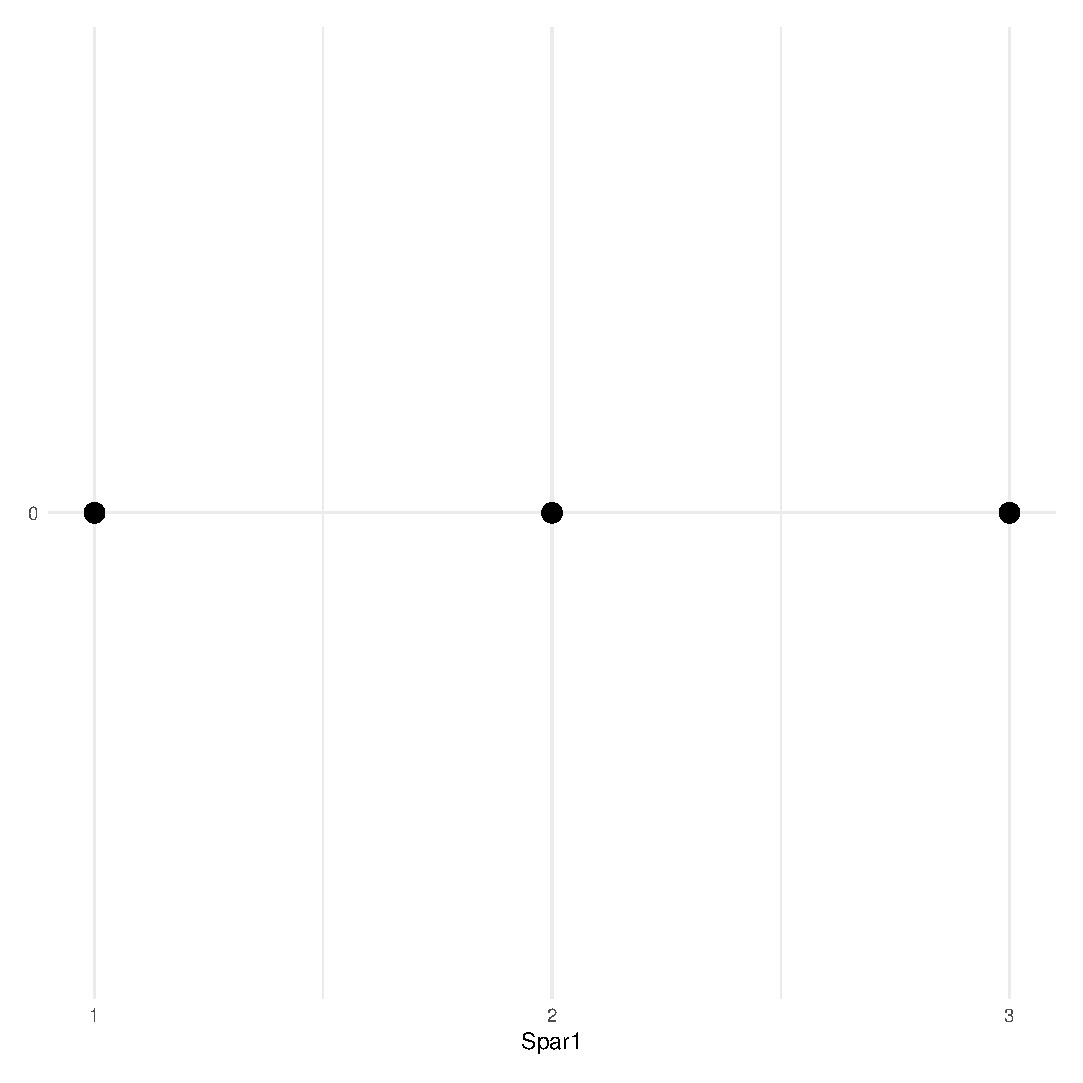
\includegraphics[width=6cm]{./images/points1}};
    \end{tikzpicture}
  }
  \only<2>{%
    \begin{textblock}{11}(-0.5,-1.5)
      {\textblockcolour{}
        \small
        \begin{tabular}{l|r|r}
        \hline
        Str & Spar1 & Spar2\\
        \hline
        ? & 1 & 1\\
        \hline
        ? & 2 & 1\\
        \hline
        ? & 3 & 1\\
        \hline
        ? & 1 & 2\\
        \hline
        ? & 2 & 2\\
        \hline
        ? & 3 & 2\\
        \hline
        ? & 1 & 3\\
        \hline
        ? & 2 & 3\\
        \hline
        ? & 3 & 3\\
        \hline
        \end{tabular}
      }
    \end{textblock}
    \begin{tikzpicture}[remember picture,overlay]
      \node[xshift=+3cm,yshift=+1.5cm] at (current page.center){%
        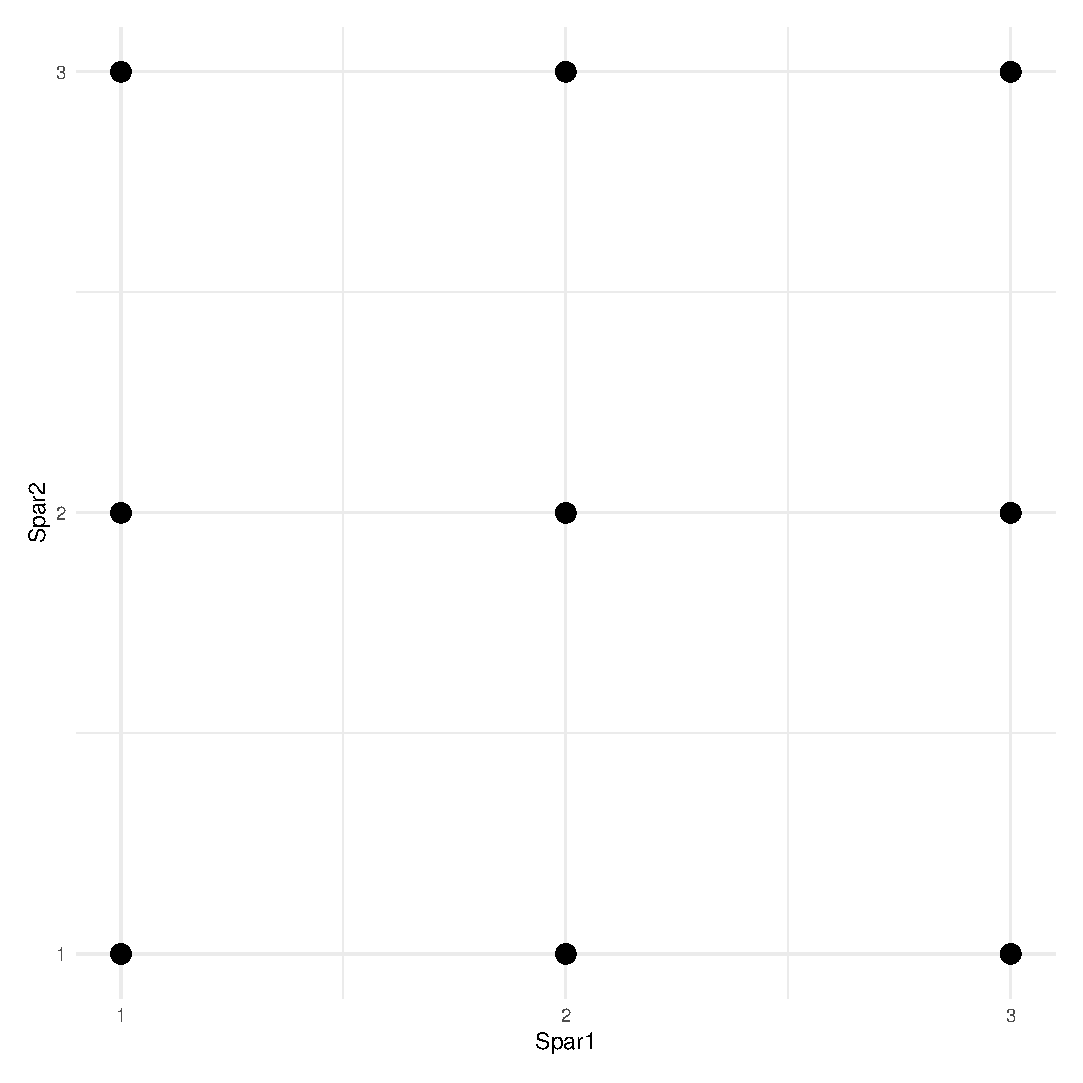
\includegraphics[width=6cm]{./images/points2}};
    \end{tikzpicture}
  }
  \only<3->{%
    \begin{textblock}{11}(-0.5,-1.5)
      {\textblockcolour{}
        \small
        \begin{tabular}{l|r|r|r}
        \hline
        Str & Spar1 & Spar2 & Rib1\\
        \hline
        ? & 1 & 1 & 1\\
        \hline
        ? & 2 & 1 & 1\\
        \hline
        ? & 3 & 1 & 1\\
        \hline
        ? & 1 & 2 & 1\\
        \hline
        ? & 2 & 2 & 1\\
        \hline
        ? & 3 & 2 & 1\\
        \hline
        ? & 1 & 3 & 1\\
        \hline
        ? & 2 & 3 & 1\\
        \hline
        ? & 3 & 3 & 1\\
        \hline
        \vdots & \vdots & \vdots & \vdots
        \end{tabular}
      }
    \end{textblock}
    \begin{tikzpicture}[remember picture,overlay]
      \node[xshift=+3cm,yshift=+1.5cm] at (current page.center){%
        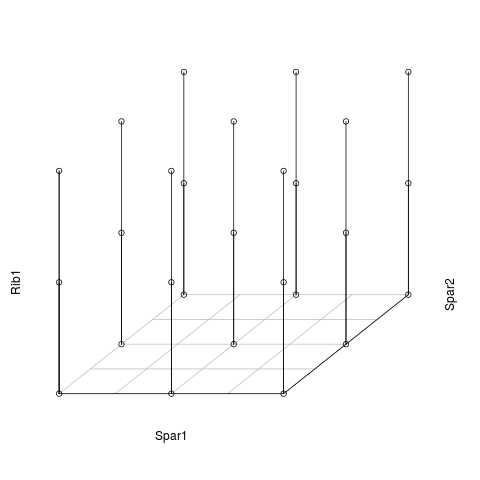
\includegraphics[width=6cm]{./images/points3}};
    \end{tikzpicture}
  }
  % Annotation
  \only<4->{
    \begin{textblock}{5}(5.5,2.5)
      {\textblockcolor{}
        That's a lot of planes! \\
        \only<5>{%
          \alert{Make a prediction:} How many planes for $d$ variables?\\
          Maybe $\approx d$? $\approx d^2$?
        }
      }
    \end{textblock}
  }
\end{frame}

% -------------------------
\framepich[0.8]{images/full_747}{
 \begin{textblock}{7}(0.0,5.7)
    {\tiny Jameson et al. (1986)}
 \end{textblock}
}

% -------------------------
\framepich[0.7]{images/titan_render}{
  \only<2>{
    \begin{textblock}{7}(0.0,4.5)
      {Simulations run\\ hours to \emph{months}}
    \end{textblock}
  }
}

% -------------------------
\begin{frame}[t]{Thought Experiment}
  Suppose our simulation ran in \emph{one second}, \\
  and we use $10$ points per dimension....

  \bigskip
  \only<2->{How long would this take to execute?\\}
  \only<3>{%
    Scaling is \emph{exponential}, i.e.
    \begin{equation*}
      \text{Time} = C^d
    \end{equation*}
  }
\end{frame}

% -------------------------
\framepicv[0.8]{images/dimensionality}{
  \only<2>{%
    \begin{textblock}{7}(3.8,3.0)
        {\textblockcolor{}
          \alert{The Curse of Dimensionality}
        }
    \end{textblock}
  }
}

% --------------------------------------------------
%% SEC: Outline
% --------------------------------------------------
\begin{frame}{Outline}
  \begin{itemize}
  \item 1. \emph{Accursed} Data
  \item 2. \emph{Accursed} Geometry
  \item 3. Lifting the Curse...
  \item 4. An Activity
  \end{itemize}
\end{frame}

% --------------------------------------------------
%% SEC: Big Data
% --------------------------------------------------
\framecard[colorgreen]{{\color{white}\hugetext{%
      \centering%
      Big Data\\
      and\\
      Dimensionality
}}}

% -------------------------
\begin{frame}{The Data Matrix}
  We've already seen one of these!

  \begin{table}
    \begin{tabular}{l|r|r|r}
      \hline
      Str & Spar1 & Spar2 & Rib1\\
      \hline
      ? & 1 & 1 & 1\\
      \hline
      ? & 2 & 1 & 1\\
      \hline
      ? & 3 & 1 & 1\\
      \hline
      ? & 1 & 2 & 1\\
      \hline
      ? & 2 & 2 & 1\\
      \hline
      ? & 3 & 2 & 1\\
      \hline
      ? & 1 & 3 & 1\\
      \hline
      ? & 2 & 3 & 1\\
      \hline
      ? & 3 & 3 & 1\\
      \hline
      \vdots & \vdots & \vdots & \vdots
    \end{tabular}
  \end{table}
\end{frame}

% -------------------------
\begin{frame}{The Data Matrix}
  % Content
  \begin{table}
    \begin{tabular}{@{}l|l|l|l@{}}
                      & Variable $1$ & $\cdots$ & Variable $d$ \\
      \hline
      Observation $1$ & $42$         & $\vdots$ & $0451$ \\
      $\vdots$        & $\vdots$     & $\vdots$ & $\vdots$
    \end{tabular}
  \end{table}
  % Annotation
  \only<2->{%
    \begin{textblock}{7}(4.0,-4.0)
      {\textblockcolor{}
        Every \alert{column} is a \alert{variable}\\
        \only<4->{Increasing dimensionality $\rhd$}
      }
    \end{textblock}
  }
  \only<3->{%
    \begin{textblock}{7}(+0.5,+1.0)
      {\textblockcolor{}
        Every \alert{row} is an \alert{observation}\\
        \only<4->{Increasing observations $\bigtriangledown$}
      }
    \end{textblock}
  }
  \only<5>{%
    \begin{textblock}{12}(-0.5,+0.0)
      {\textblockcolor{}
        \LARGE Both contribute to `Big Data'
      }
    \end{textblock}
  }
\end{frame}

% -------------------------
\framecard[colorblue]{{\color{white}%

``The trend today is towards more observations \emph{but even more so},
    \alert{to radically larger numbers of variables} – voracious, automatic,
    systematic collection of hyper-informative detail about each observed
    instance.''

    \bigskip
    -- David Donoho, 2000\\
    \tiny (Emphasis added)

}}

% -------------------------
\begin{frame}{How Big is our Data?}
  \begin{itemize}
  \item<1-> How many entries in a data matrix?\\
    \visible<2->{\alert<2>{%
      -- Observations $\times$ Dimensionality
    }}

    \bigskip
  \item<3-> How many Observations needed for Dimensionality?\\
    \visible<4->{\alert<4>{%
      -- Exponential in Dimensionality\textsuperscript{*}
    }}

    \bigskip
  \item<5-> How many hard drives will we need?!

    \bigskip
  \item<6> What's so special about high dimensionality?
  \end{itemize}
\end{frame}

% --------------------------------------------------
%% SEC: High-dimensional geometry
% --------------------------------------------------
\framecard[colorgreen]{{\color{white}\hugetext{%
      \centering%
      Weird Facts\\
      about\\
      High-\\
      Dimensional\\
      Geometry
}}}

% -------------------------
\begin{frame}{Fact 1}
  Basic solids defy intuition
\end{frame}

% -------------------------
\begin{frame}{Sketching Solids}
  Hyperspheres and Hypercubes
\end{frame}

% -------------------------
\begin{frame}[plain]
  \begin{textblock}{7}(-0.5,-3.5)
    {\textblockcolor{}
      Hypercube on $[-\f12,+\f12]^d$\\
      Hypersphere of radius $1$\\
      Which is bigger for $d = 2$?
    }
  \end{textblock}
\end{frame}

% -------------------------
\framepich[1.0]{images/box_in_sphere1}{
  % Annotation
  \begin{textblock}{2}(+0.5,+4.0)
    {\textblockcolor{}
      $d = 2$
    }
  \end{textblock}

  % Footer
  \begin{textblock}{7}(0.0,5.7)
    {\tiny By Venkatesan Guruswami}
  \end{textblock}
}

% -------------------------
\framepich[1.0]{images/box_in_sphere2}{
  % Annotation
  \begin{textblock}{2}(+0.5,+4.0)
    {\textblockcolor{}
      $d = 2$
    }
  \end{textblock}

  \begin{textblock}{2}(+4.7,+4.0)
    {\textblockcolor{}
      $d = 4$
    }
  \end{textblock}

 \begin{textblock}{7}(0.0,5.7)
    {\tiny By Venkatesan Guruswami}
 \end{textblock}
}

% -------------------------
\framepich[1.0]{images/box_in_sphere3}{
  % Annotation
  \begin{textblock}{2}(+0.5,+4.0)
    {\textblockcolor{}
      $d = 2$
    }
  \end{textblock}

  \begin{textblock}{2}(+4.7,+4.0)
    {\textblockcolor{}
      $d = 4$
    }
  \end{textblock}

  \begin{textblock}{2}(+9.0,+4.0)
    {\textblockcolor{}
      $d \to \infty$
    }
  \end{textblock}

 \begin{textblock}{7}(0.0,5.7)
    {\tiny By Venkatesan Guruswami}
 \end{textblock}
}

% -------------------------
\begin{frame}{Fact 2}
  The hypersphere has vanishing interior
\end{frame}

% -------------------------
\begin{frame}{Unit Hypersphere Volume}
  \begin{equation*} \begin{aligned}
      HV &= \frac{\pi ^ {d / 2}}{\Gamma(d / 2 + 1)}\\
      \visible<2>{%
        &= \int\cdots\int \alert{r^{d-1}}\,
           T(\varphi_{1},\dots,\varphi_{d-1})\,
           dr d\varphi_{1}\cdots d\varphi_{d-1}
      }
  \end{aligned} \end{equation*}
\end{frame}

% -------------------------
\framepicv[0.8]{images/surface_density}{}

% -------------------------
\begin{frame}{Fact 3}
  Johnson-Lindenstrauss Lemma....
\end{frame}

% -------------------------
\begin{frame}{We Will Study:}
  \underline{Claim}: For any $0<\epsilon<1$ and $n\in\mathbb{Z}_{>0}$, let
  $k\in\mathbb{Z}_{>0}$ such that

  \begin{equation*}
    k \geq C \frac{\log(n)}{\epsilon^2},
  \end{equation*}

  \noindent then for all sets of points $V\subset\R{d}$, there is a projection
  $P_k:\R{d}\to\R{k}$ such that, for all $u,v\in V$, we have

    \begin{equation*}
      \alert<2>{(1 - \epsilon)\|\vu - \vv\|^2 \leq \alpha\|P_k(\vu) - P_k(\vv)\|^2 \leq %
      (1 + \epsilon)\|\vu - \vv\|^2
}    \end{equation*}
\end{frame}

% JL: Distance
% -------------------------
\begin{frame}{}
  % Content
  \only<-5>{%
    \begin{equation*} \begin{aligned}
        (1 - \alert<3>{\epsilon})(\alert<2>{\text{Distance}})^2 &\leq %
          \alpha(\alert<4,5>{\text{Projected Distance}})^2 \\
        &\, \\
        \alpha(\alert<4,5>{\text{Projected Distance}})^2 &\leq %
          (1 + \alert<3>{\epsilon})(\alert<2>{\text{Distance}})^2\\
    \end{aligned} \end{equation*}
  }%
  % Annotation
  \visible<2-5>{%
    \begin{textblock}{3}(+1.5,-5.7)
      {\textblockcolor{}
        \centering%
        \only<2>{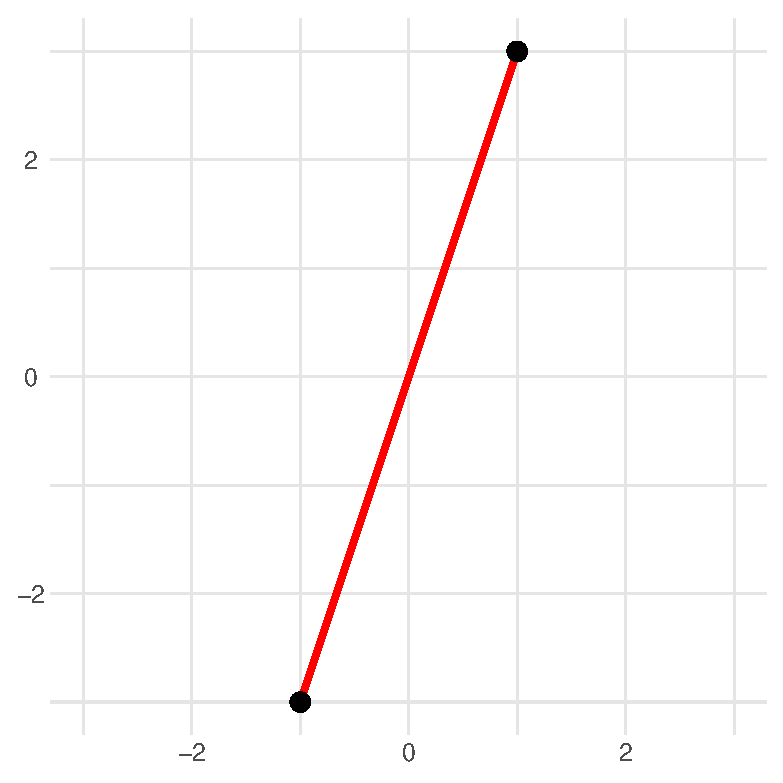
\includegraphics[width=1.0\textwidth]{./images/proj0_alert}}
        \only<3-5>{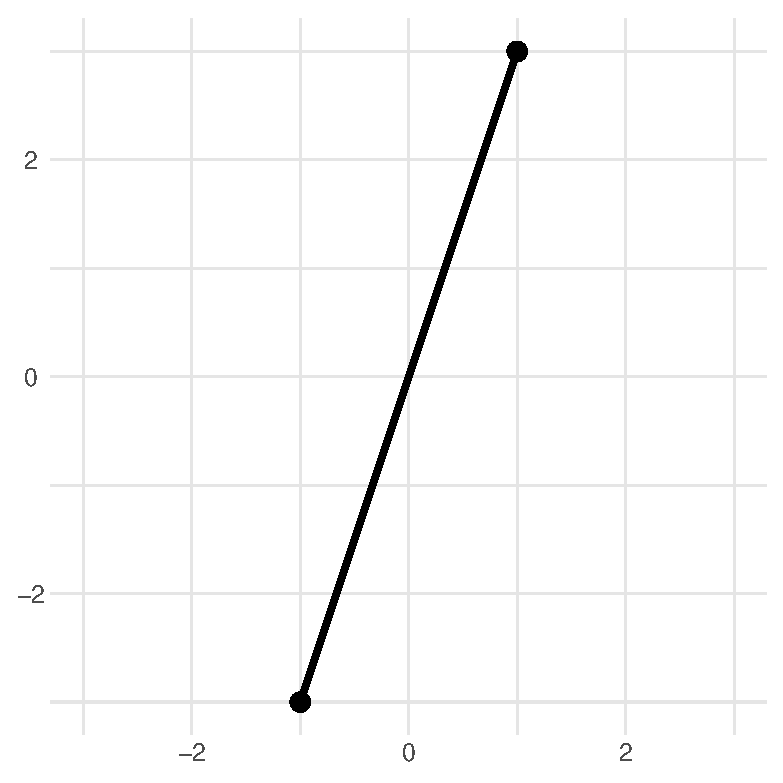
\includegraphics[width=1.0\textwidth]{./images/proj0}}
      }
    \end{textblock}
  }
  \visible<3-5>{%
    \begin{textblock}{3}(+5.5,-4.0)
      {\textblockcolor{}
        \alert<3>{$\epsilon$ is \emph{small}}
      }
    \end{textblock}
  }
  \visible<4-5>{%
    \begin{textblock}{3}(-0.5,+0.0)
      {\textblockcolor{}
        \centering%
        \only<4>{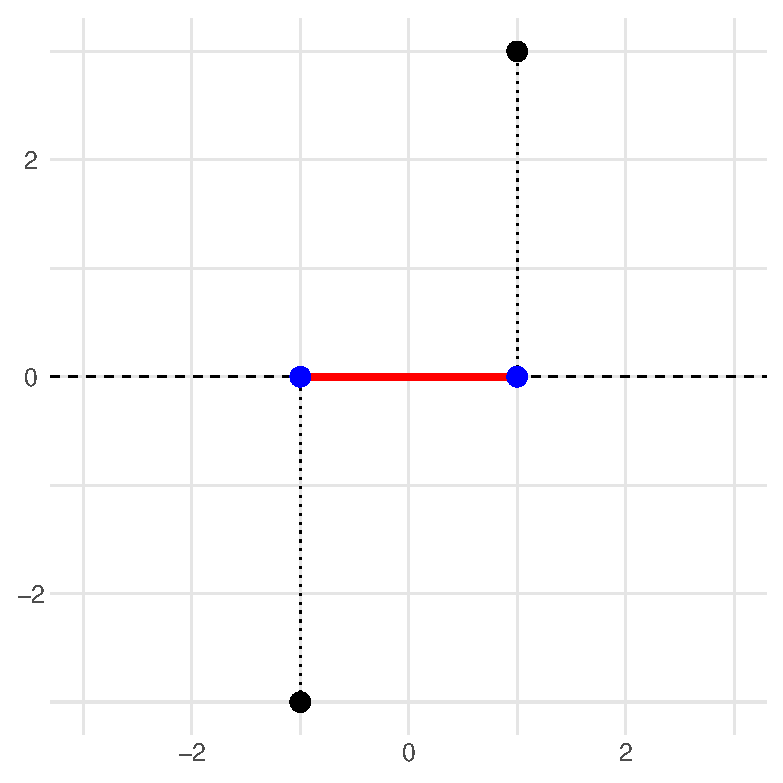
\includegraphics[width=1.0\textwidth]{./images/proj1_alert}}
        \only<5>{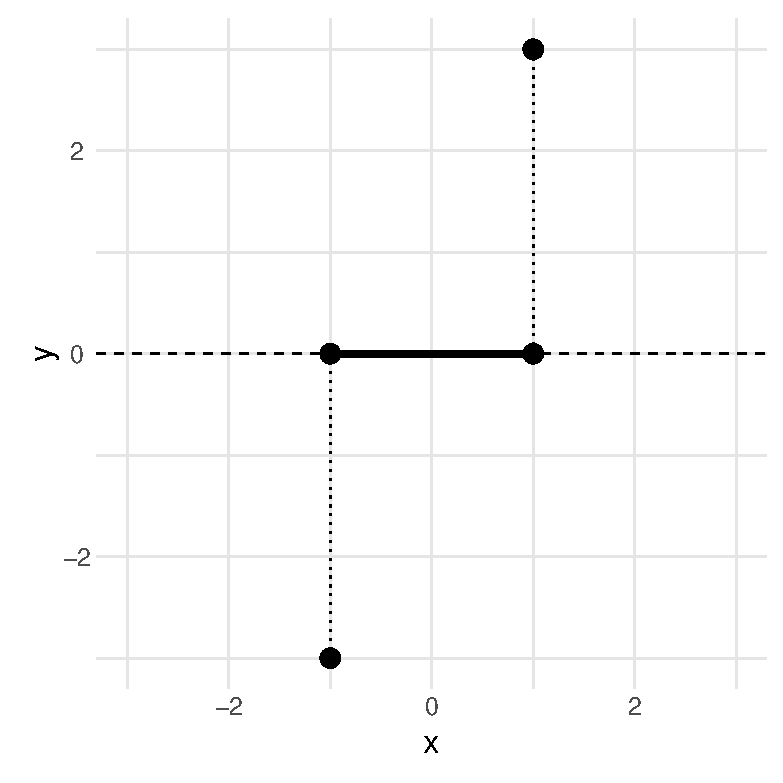
\includegraphics[width=1.0\textwidth]{./images/proj1}}
      }
    \end{textblock}
  }
  \visible<5-5>{%
    \begin{textblock}{3}(+3.0,+0.0)
      {\textblockcolor{}
        \centering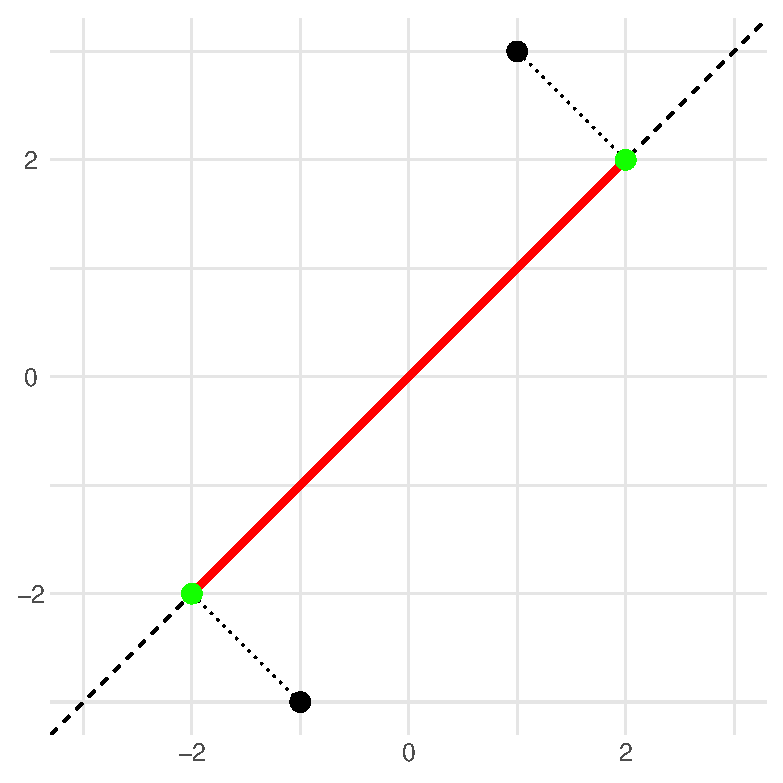
\includegraphics[width=1.0\textwidth]{./images/proj2_alert}
      }
    \end{textblock}
  }
\end{frame}

% JL: Projections
% -------------------------
\begin{frame}[t]{}
  % Content
  \begin{equation*}
    (1 - \epsilon)\|\vu - \vv\|^2 \leq %
    \alert{\alpha}\|P_{\alert{k}}(\vu) - P_{\alert{k}}(\vv)\|^2 \leq %
    (1 + \epsilon)\|\vu - \vv\|^2
  \end{equation*}
  % Annotation
  \visible<2->{%
    \begin{textblock}{6}(+2.5,-0.5)
      {\textblockcolor{}
        \centering%
        \only<2>{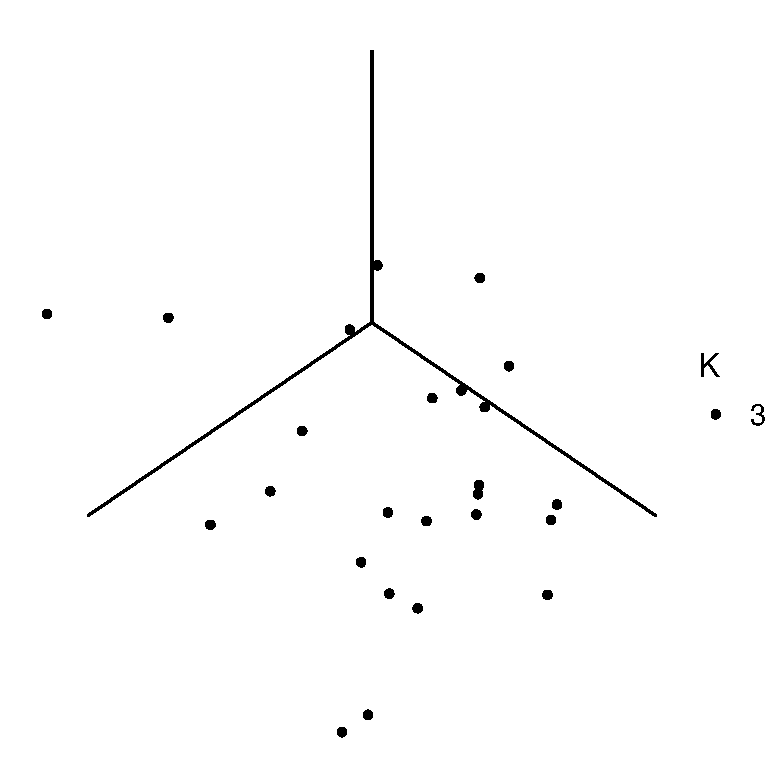
\includegraphics[width=1.0\textwidth]{./images/dim_proj3}}
        \only<3>{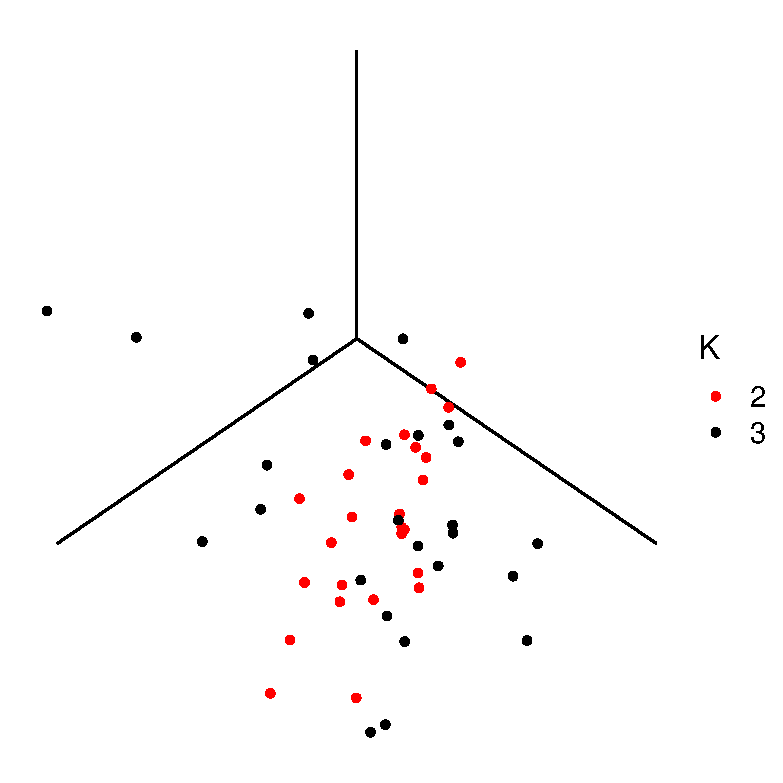
\includegraphics[width=1.0\textwidth]{./images/dim_proj2}}
        \only<4>{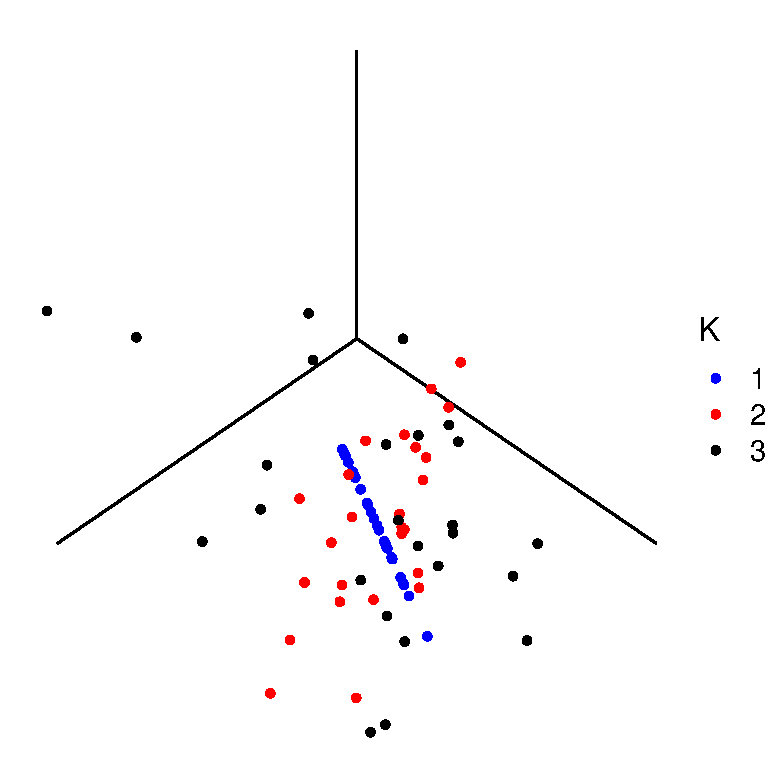
\includegraphics[width=1.0\textwidth]{./images/dim_proj1}}
      }
    \end{textblock}
  }
\end{frame}

% JL: Dimensionality
% -------------------------
\begin{frame}{}
  % Content
  \begin{equation*}
    \alert<2>{k} \geq C\frac{\log(\alert<3>{n})}{\alert<4>{\epsilon}^2}
  \end{equation*}
  % Annotation
  \visible<2->{%
    \begin{textblock}{4}(+0.0,-3.5)
      {\textblockcolor{}
        $k$ is the projection dimension
      }
    \end{textblock}
  }
  \visible<3->{%
    \begin{textblock}{4}(+0.0,+2.0)
      {\textblockcolor{}
        $n$ is the number of observations
      }
    \end{textblock}
  }
  \visible<4->{%
    \begin{textblock}{4}(+7.0,+2.0)
      {\textblockcolor{}
        $\epsilon$ is the desired error
      }
    \end{textblock}
  }
  \visible<5->{%
    \begin{textblock}{4.5}(+7.0,-3.5)
      {\textblockcolor{}
        Dimensionality is\\
        \emph{curiously absent!}
      }
    \end{textblock}
  }
\end{frame}

% JL: Example
% -------------------------
\begin{frame}[fragile]{JL: Example}
Example: Gene expression levels for tumor types BRCA, KIRC, COAD, LUAD and PRAD.

\bigskip
  \begin{lstlisting}
## Gene data from UCI
dim(gene_data)
#       Obs,  Dim
> [1]   801 20531
  \end{lstlisting}

  \bigskip
  Note: This code on GitHub: https://github.com/zdelrosario/hyperspace
\end{frame}

% -------------------------
\begin{frame}[fragile]{JL: Example}
  \begin{lstlisting}
C <- 2                 # Over-samping
eps <- 0.1             # 10% distort
n <- dim(gene_data)[1] # Observations
d <- dim(gene_data)[2] # Dimension

k <-  ceiling(C * log(n) / eps ^ 2)
k
> 1338 (6.5% of 20531)
  \end{lstlisting}
\end{frame}

% -------------------------
\begin{frame}[fragile]{JL: Example}
  \begin{lstlisting}
## Randomly project
P_k <- random_projection(k x d)
projected_data = gene_data %*% P_k
  \end{lstlisting}
\end{frame}

% -------------------------
\begin{frame}[fragile]{JL: Example}
  \begin{lstlisting}
eps
# Requested distortion
>    10%
quantile(relative_difference)
# Quantile
>      0%     25%    50%    75%   100%
# Realized distortion
> -7.784% -1.193% 0.082% 1.344% 8.139%
  \end{lstlisting}
\end{frame}

% --------------------------------------------------
%% SEC: Dimension Reduction
% --------------------------------------------------
\framecard[colorgreen]{{\color{white}\hugetext{%
      \centering%
      Lifting\\
      the\\
      Curse
}}}

% -------------------------
\begin{frame}{Dimension Reduction}
  \huge\underline{Idea:} Find \emph{low-dimensional} structure in data
\end{frame}

% -------------------------
\begin{frame}{Ex: Low-Dimensional Structure}
  Example: FAA Aircraft characteristic database

  \bigskip
  \begin{tabular}{@{}ll@{}}
    Variable & Description \\
    \hline
    wingspan    & Wingspan [ft] \\
    length      & Length [ft] \\
    %% tail\_height & Tail height [ft] \\
    %% cmg         & Cockpit-to-main gear [ft] \\
    %% mgw         & Main gear width [ft] \\
    mtow        & Maximum take-off weight [lbs] \\
    approach\_speed & Approach speed [kts]
  \end{tabular}
\end{frame}

% -------------------------
\begin{frame}{Ex: Low-Dimensional Structure}
  \begin{figure}
    \centering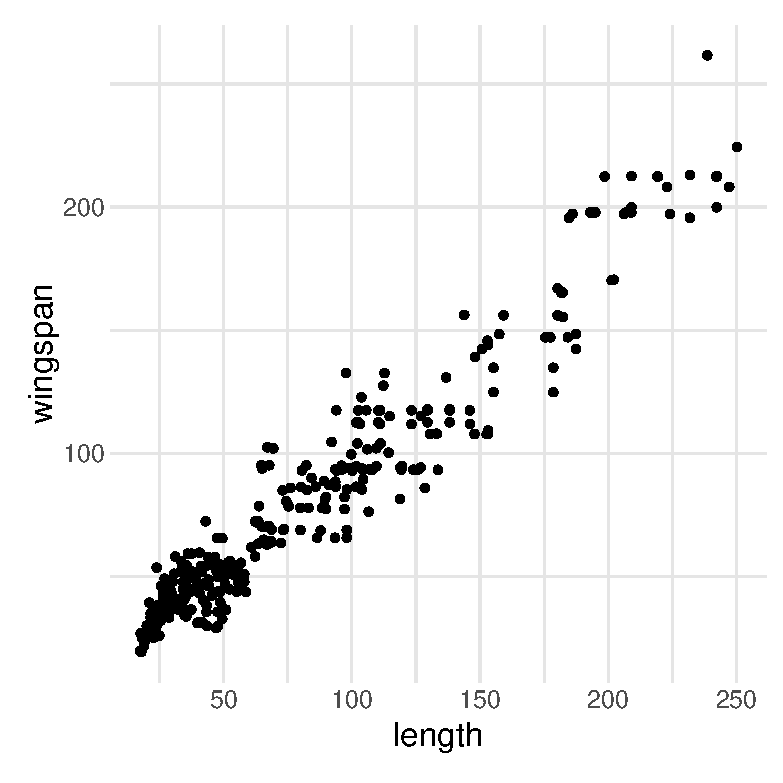
\includegraphics[width=0.7\textwidth]{./images/faa_wingspan_v_length}
  \end{figure}
\end{frame}

% -------------------------
\begin{frame}{Ex: Low-Dimensional Structure}
  \begin{figure}
    \centering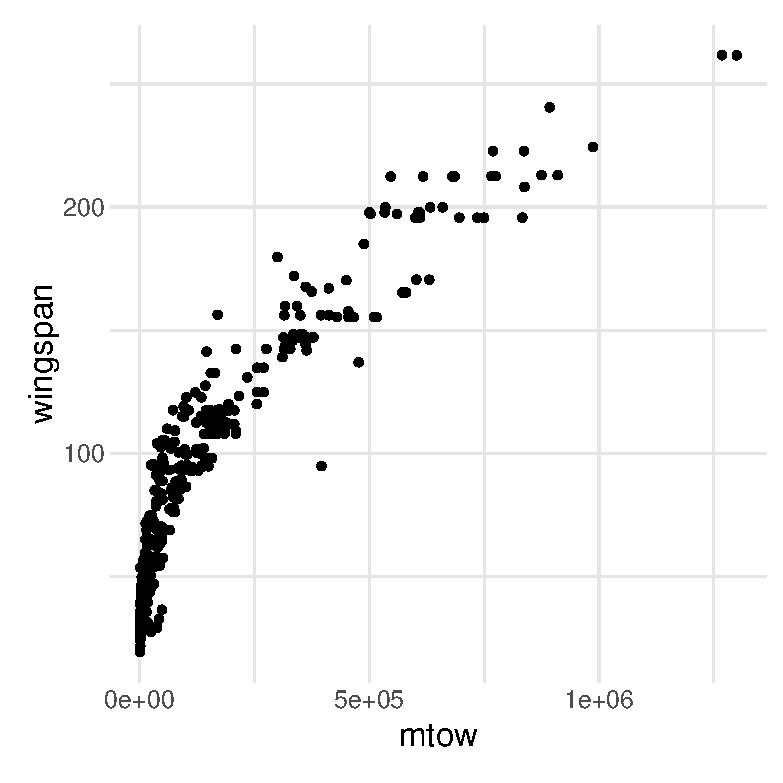
\includegraphics[width=0.7\textwidth]{./images/faa_wingspan_v_mtow}
  \end{figure}
\end{frame}

% -------------------------
\begin{frame}{Ex: Low-Dimensional Structure}
  \begin{figure}
    \centering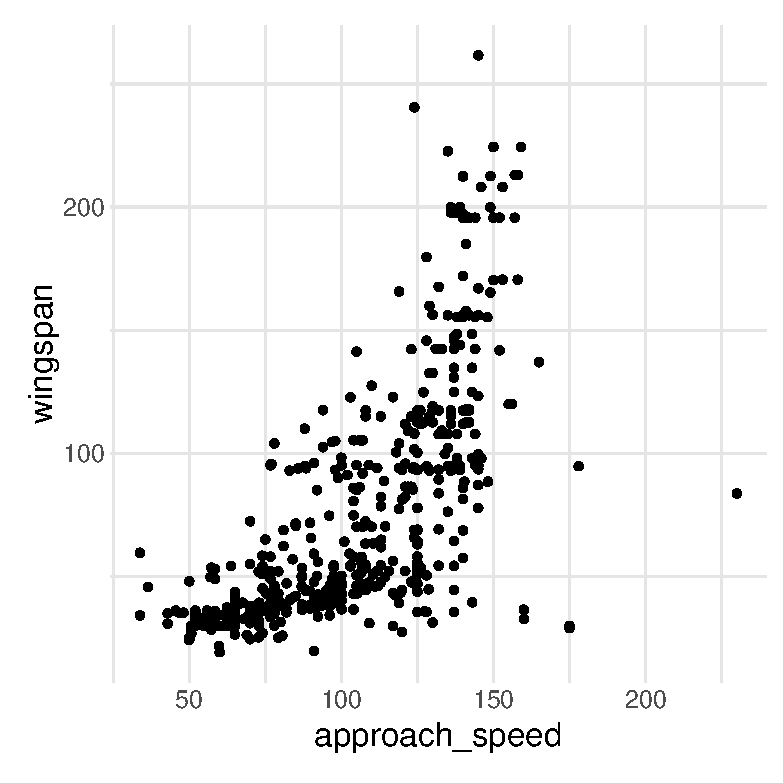
\includegraphics[width=0.7\textwidth]{./images/faa_wingspan_v_approach_speed}
  \end{figure}
\end{frame}

% -------------------------
\begin{frame}{Ex: Scatterplot Matrix}
  \begin{figure}
    \centering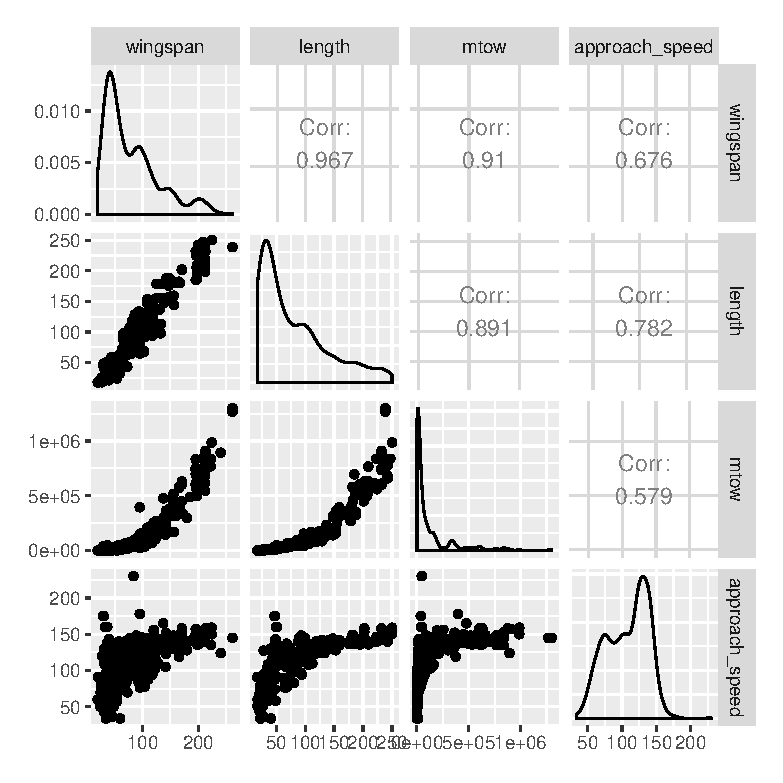
\includegraphics[width=0.7\textwidth]{./images/faa_min_scatter}
  \end{figure}
\end{frame}

% -------------------------
\begin{frame}{Ex: Scatterplot Matrix, log}
  \begin{figure}
    \centering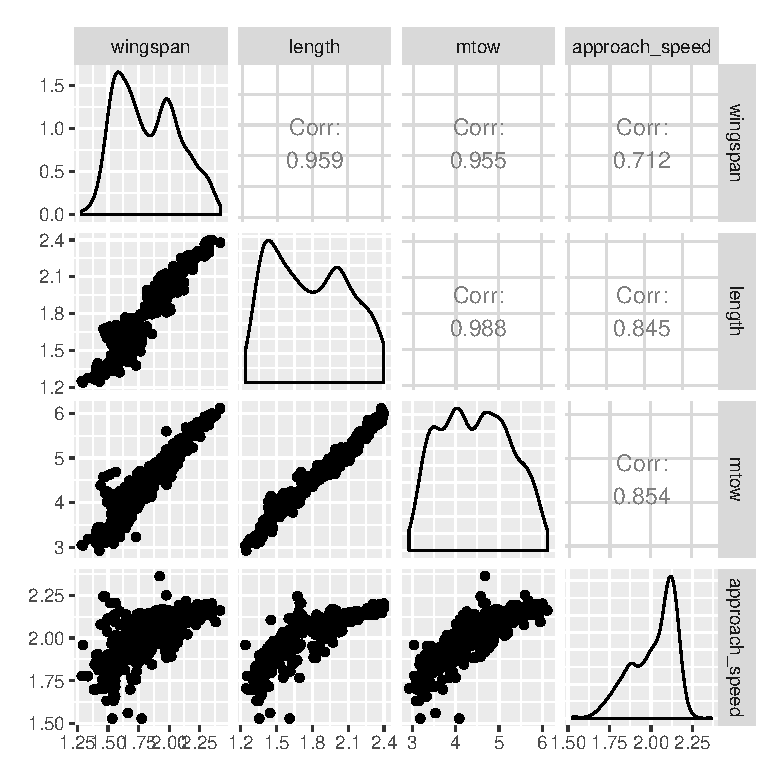
\includegraphics[width=0.7\textwidth]{./images/faa_min_scatter_log}
  \end{figure}
\end{frame}

% -------------------------
\begin{frame}{Finding Low-Dimensional Structure}
  \begin{itemize}
  \item Johnson-Lindenstrauss -- Random!
  \item Important directions -- Data-informed
  \end{itemize}
\end{frame}

% -------------------------
\begin{frame}{Important Directions}
  \huge\underline{Idea:} Find directions that capture variability
\end{frame}

% -------------------------
\framepicv[1.0]{images/pca1}{}
\framepicv[1.0]{images/pca2}{}
\framepicv[1.0]{images/pca3}{
  \visible<2>{
    \begin{textblock}{7}(4.8,4.0)
      {\textblockcolor{}
        Direction \alert{from data} \\
        Called \emph{principal component analysis}
      }
    \end{textblock}
  }
}

% -------------------------
\begin{frame}[fragile]{Applied to FAA Data}
  \begin{lstlisting}
df_faa_pca <- df_faa %>%
    tidy_pca(
        wingspan, length,
        mtow, approach_speed
    )
df_faa_pca %>%
    pull(pc_frac)
> | k |  Var |  Frac |
> --------------------
> | 1 | 1.87 | 0.64% |
> | 2 | 0.66 | 0.86% |
> | 3 | 0.25 | 0.95% |
> | 4 | 0.15 | 1.00% |
  \end{lstlisting}
\end{frame}

% -------------------------
\begin{frame}{Applied to FAA Data}
  \begin{figure}
    \centering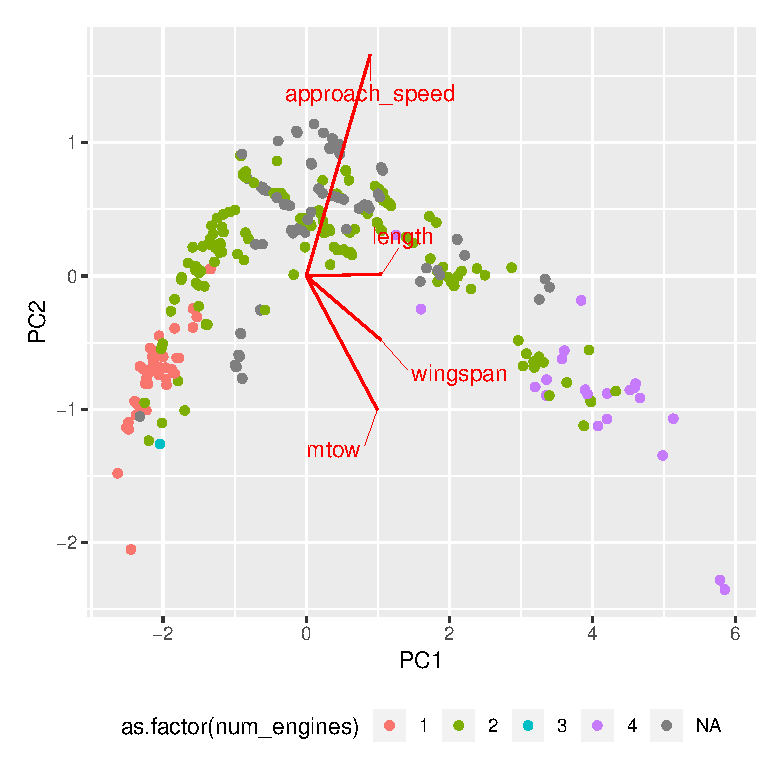
\includegraphics[width=0.7\textwidth]{./images/faa_min_pca_plot}
  \end{figure}
\end{frame}

% --------------------------------------------------
%% SEC: Activity
% --------------------------------------------------
\framecard[colorgreen]{{\color{white}\hugetext{%
      \centering%
      Activity!
}}}

\end{document}
